\chapter{Resultados e discussão}\label{cap:resultados}

Este capítulo apresenta os resultados da avaliação descrita no Capítulo~\ref{cap:metodologia}: primeiro o panorama agregado entre os seis sistemas comparáveis (\textit{basic}, \textit{local} e \textit{drift}, nos níveis de comunidade 1 e 2), em seguida o desempenho por doença, a investigação dirigida ao comportamento do modo \textit{drift} nas duas direções de erro e, por fim, a análise qualitativa de grafos. Os sistemas S5 e S6 (modo \textit{global}) não constam das comparações por não terem sido concluídos de forma confiável, pelos motivos expostos na Seção~\ref{sec:met-desenho}.

\section{Panorama agregado}\label{sec:res-panorama}

A Tabela~\ref{tab:res-metricas-gerais} reúne as métricas agregadas dos seis sistemas avaliados. O modo \textit{drift} (S7 e S8) obtém o maior F1 macro entre os seis sistemas, com destaque para S8 (nível de comunidade 2), que alcança 0,798 contra 0,745 de S7 (nível 1). Os modos \textit{basic} e \textit{local} apresentam F1 macro entre 0,681 e 0,743, inferior ao do \textit{drift} em todas as quatro configurações.

\begin{table}[!htbp]
\centering
\caption[Métricas agregadas dos seis sistemas avaliados]{Métricas agregadas dos seis sistemas avaliados (537 prontuários; 531 respostas válidas em S8).}
\label{tab:res-metricas-gerais}
\begin{tabular}{lccccc>{\columncolor{colunaDestaque}}cc}
\toprule
Sistema & Modo & Nível & EM & P$_{\text{macro}}$ & R$_{\text{macro}}$ & F1$_{\text{macro}}$ & F1$_{\text{micro}}$ \\
\midrule
S1 & \chip{modoBasic}\textit{basic} & 1 & 0,575 & 0,783 & 0,613 & 0,681 & 0,738 \\
S2 & \chip{modoBasic}\textit{basic} & 2 & 0,566 & \tsecond{0,852} & 0,592 & 0,689 & 0,721 \\
S3 & \chip{modoLocal}\textit{local} & 1 & 0,581 & \tfirst{0,858} & 0,635 & 0,718 & 0,750 \\
S4 & \chip{modoLocal}\textit{local} & 2 & 0,587 & \tfirst{0,858} & 0,672 & 0,743 & 0,739 \\
S7 & \chip{modoDrift}\textit{drift}  & 1 & \tsecond{0,596} & 0,648 & \tsecond{0,946} & \tsecond{0,745} & \tsecond{0,825} \\
\rowcolor{linhaDestaque}S8 & \chip{modoDrift}\textit{drift}  & 2 & \tfirst{0,625} & 0,707 & \tfirst{0,948} & \cellcolor{colunaDestaque}\tfirst{0,798} & \tfirst{0,850} \\
\bottomrule
\end{tabular}
\par\smallskip{\footnotesize Fonte: elaborado pelo autor a partir de \texttt{metricas\_parcial\_sem\_global.csv}. EM: acurácia de correspondência exata; P, R: precisão e revocação. \tfirst{Vermelho} e \tsecond{azul}: melhor e segundo melhor valor de cada coluna; em destaque, o melhor sistema e a métrica principal (F1 macro).}
\end{table}

O padrão mais relevante da Tabela~\ref{tab:res-metricas-gerais} é a assimetria entre precisão e revocação no modo \textit{drift}: revocação macro de 94,6\% (S7) e 94,8\% (S8), contra 59,2\% a 67,2\% em \textit{basic} e \textit{local}, ao custo de precisão macro de 64,8\% a 70,7\%, inferior aos 78,3\% a 85,8\% dos demais modos. A Figura~\ref{fig:res-f1-sistemas} ilustra essa troca: o F1 macro mais alto do \textit{drift} é sustentado por uma cobertura muito superior, e não por acertos mais seletivos.

\begin{figure}[!htbp]
\centering
% Barras horizontais com rótulo interno e legenda em quadro arredondado,
% no estilo de OA-RAG (arXiv:2610.36335). Uma cor por modo de busca.
\begin{tikzpicture}[x=1cm, y=1cm, font=\footnotesize]
\def\X{1.75}\def\W{3.75}\def\G{0.45}\def\H{0.27}
\node[anchor=south, draw=black!40, line width=0.4pt, rounded corners=2pt, inner xsep=4pt, inner ysep=2pt, font=\scriptsize]
  at ({\X+1.5*\W+\G},0.42) {\chip{modoBasic}\textit{basic}\hspace{8pt}\chip{modoLocal}\textit{local}\hspace{8pt}\chip{modoDrift}\textit{drift}};
\foreach \k/\tit in {0/Precisão macro, 1/Revocação macro, 2/F1 macro}{
  \pgfmathsetmacro{\x}{\X+\k*(\W+\G)}
  \node[font=\footnotesize\bfseries, anchor=base, inner sep=1pt] at ({\x+\W/2},0.0) {\tit};
  \foreach \t/\lab in {0/0, 0.25/{}, 0.5/{0,5}, 0.75/{}, 1/1}{
    \draw[black!10, line width=0.4pt] ({\x+\W*\t},-0.15) -- ({\x+\W*\t},-3.20);
    \node[anchor=north, inner sep=1.5pt, text=black!65, font=\scriptsize] at ({\x+\W*\t},-3.20) {\lab};
  }
  \draw[black!45, line width=0.4pt] (\x,-3.20) -- ({\x+\W},-3.20);
}
\foreach \s/\n/\c/\y/\p/\r/\f in {
    S1/1/modoBasic/-0.40/0.783/0.613/0.681,
    S2/2/modoBasic/-0.78/0.852/0.592/0.689,
    S3/1/modoLocal/-1.43/0.858/0.635/0.718,
    S4/2/modoLocal/-1.81/0.858/0.672/0.743,
    S7/1/modoDrift/-2.46/0.648/0.946/0.745,
    S8/2/modoDrift/-2.84/0.707/0.948/0.798}{
  \node[anchor=east, inner sep=0pt] at ({\X-0.08},\y) {\s\ {\scriptsize\color{black!60}(nível \n)}};
  \foreach \k/\v in {0/\p, 1/\r, 2/\f}{
    \pgfmathsetmacro{\x}{\X+\k*(\W+\G)}
    \path[fill=\c, draw=white, line width=0.45pt] (\x,{\y+\H/2}) rectangle ({\x+\W*\v},{\y-\H/2});
    \node[anchor=east, inner sep=2pt, text=white, font=\scriptsize] at ({\x+\W*\v},\y)
      {\pgfmathprintnumber[fixed, precision=3, fixed zerofill, use comma]{\v}};
  }
}
\foreach \ys in {-1.105, -2.135}{\draw[black!25, line width=0.4pt] (0.2,\ys) -- ({\X+3*\W+2*\G},\ys);}
\end{tikzpicture}
\caption[Precisão, revocação e F1 macro por sistema]{Precisão, revocação e F1 macro por sistema.}
\label{fig:res-f1-sistemas}
\par\smallskip{\footnotesize Fonte: elaborado pelo autor a partir de \texttt{metricas\_parcial\_sem\_global.csv}.}
\end{figure}

\section{Desempenho por doença}\label{sec:res-por-doenca}

A Figura~\ref{fig:res-f1-doenca} compara o F1 por doença entre os modos \textit{basic} (referência sem uso estruturado do grafo), \textit{local} e \textit{drift} nos dois níveis de comunidade avaliados: S1, S3 e S7, no nível 1 (painel a), e S2, S4 e S8, no nível 2 (painel b). O padrão confirma, com ressalvas, a distinção entre doenças de marcador binário claro e doenças de inferência indireta. Em cirrose hepática e hipertensão portal, doenças que dependem de inferência a partir de múltiplos achados dispersos no texto, o ganho do \textit{drift} sobre o \textit{basic} é o maior nos dois níveis: 18,1 e 19,7 pontos de F1 no nível 1, e 23,1 e 22,1 pontos no nível 2. Em esteatose hepática e hepatite C, cujo texto costuma registrar um exame ou laudo objetivo, o ganho é menor, por efeito-teto (o \textit{basic} já desempenha bem nessas classes): 5,4 e 9,0 pontos no nível 1, e 9,6 e 12,7 no nível 2. A esquistossomose, apesar de também depender de inferência indireta, tem ganho modesto nos dois níveis (5,0 e 8,6 pontos), semelhante ao das doenças de marcador direto.

As duas exceções observadas no nível 1 não se repetem no nível 2. Na hepatite B, o \textit{drift} fica ligeiramente abaixo do \textit{basic} no nível 1 (0,851 contra 0,864), mas o supera no nível 2 (0,927 contra 0,857). Na hemorragia digestiva alta (HDA), o \textit{drift} não supera o \textit{local} no nível 1 (0,457 contra 0,485) e, no nível 2, é o melhor dos três modos, mas com F1 ainda baixo (0,486). Em ambos os níveis, a HDA tem o pior desempenho entre as sete doenças avaliáveis, apesar de o termo literal estar presente na maior parte dos prontuários positivos, o que é consistente com o mecanismo de confusão anatômica investigado e estatisticamente confirmado na Seção~\ref{sec:res-investigacao-erro}. No nível 2, portanto, o \textit{drift} obtém o maior F1 em todas as doenças, e a vantagem continua concentrada nas de evidência indireta.

\begin{figure}[!htbp]
\centering
% Barra proporcional dentro de cada célula, como no painel de acurácia de
% OA-RAG (arXiv:2610.36335); setas de ganho/perda (\gain/\loss) do mesmo artigo.
\resizebox{\textwidth}{!}{%
\begin{tikzpicture}[x=1cm, y=1cm, font=\footnotesize]
\def\X{3.95}\def\CW{3.05}\def\GX{0.22}\def\RH{0.44}\def\BH{0.27}
\foreach \k/\tit/\c in {0/{S1 (\textit{basic})}/modoBasic, 1/{S3 (\textit{local})}/modoLocal, 2/{S7 (\textit{drift})}/modoDrift}{
  \node[font=\footnotesize\bfseries, anchor=base, inner sep=1pt] at ({\X+\k*(\CW+\GX)+\CW/2},0.08) {\chip{\c}\tit};
}
\node[font=\footnotesize\bfseries, anchor=base, inner sep=1pt] at ({\X+3*(\CW+\GX)+0.62},0.08) {$\Delta$};
\draw[black!45, line width=0.4pt] (-0.15,-0.08) -- ({\X+3*(\CW+\GX)+1.45},-0.08);
\foreach \i/\nome/\a/\b/\d/\best/\delta in {
    1/Cirrose hepática/0.627/0.602/0.808/2/{\gain{18,1}},
    2/Esquistossomose/0.691/0.735/0.741/2/{\gain{5,0}},
    3/Hepatite C/0.779/0.782/0.869/2/{\gain{9,0}},
    4/Hepatite B/0.864/0.882/0.851/1/{\loss{1,3}},
    5/Esteatose hepática/0.882/0.869/0.936/2/{\gain{5,4}},
    6/Hipertensão portal/0.700/0.726/0.897/2/{\gain{19,7}},
    7/{Hemorragia digestiva alta}/0.406/0.485/0.457/1/{\gain{5,1}}}{
  \pgfmathsetmacro{\y}{-0.08-\i*\RH+\RH/2}
  \node[anchor=east, inner sep=0pt] at ({\X-0.10},\y) {\nome};
  \foreach \k/\v/\c in {0/\a/modoBasic, 1/\b/modoLocal, 2/\d/modoDrift}{
    \pgfmathsetmacro{\x}{\X+\k*(\CW+\GX)}
    \fill[black!5] (\x,{\y+\BH/2}) rectangle ({\x+\CW},{\y-\BH/2});
    \path[fill=\c, draw=white, line width=0.45pt] (\x,{\y+\BH/2}) rectangle ({\x+\CW*\v},{\y-\BH/2});
    \ifnum\k=\best\draw[black!75, line width=0.7pt] (\x,{\y+\BH/2}) rectangle ({\x+\CW*\v},{\y-\BH/2});\fi
    \node[anchor=east, inner sep=2pt, text=white, font=\scriptsize] at ({\x+\CW*\v},\y)
      {\ifnum\k=\best\bfseries\fi\pgfmathprintnumber[fixed, precision=3, fixed zerofill, use comma]{\v}};
  }
  \node[anchor=west, inner sep=0pt, font=\scriptsize] at ({\X+3*(\CW+\GX)+0.10},\y) {\delta};
}
\draw[black!45, line width=0.4pt] (-0.15,{-0.08-7*\RH}) -- ({\X+3*(\CW+\GX)+1.45},{-0.08-7*\RH});
\end{tikzpicture}}\\[2pt]
{\footnotesize (a) Nível 1}
\\[8pt]
\resizebox{\textwidth}{!}{%
\begin{tikzpicture}[x=1cm, y=1cm, font=\footnotesize]
\def\X{3.95}\def\CW{3.05}\def\GX{0.22}\def\RH{0.44}\def\BH{0.27}
\foreach \k/\tit/\c in {0/{S2 (\textit{basic})}/modoBasic, 1/{S4 (\textit{local})}/modoLocal, 2/{S8 (\textit{drift})}/modoDrift}{
  \node[font=\footnotesize\bfseries, anchor=base, inner sep=1pt] at ({\X+\k*(\CW+\GX)+\CW/2},0.08) {\chip{\c}\tit};
}
\node[font=\footnotesize\bfseries, anchor=base, inner sep=1pt] at ({\X+3*(\CW+\GX)+0.62},0.08) {$\Delta$};
\draw[black!45, line width=0.4pt] (-0.15,-0.08) -- ({\X+3*(\CW+\GX)+1.45},-0.08);
\foreach \i/\nome/\a/\b/\d/\best/\delta in {
    1/Cirrose hepática/0.571/0.626/0.802/2/{\gain{23,1}},
    2/Esquistossomose/0.679/0.702/0.765/2/{\gain{8,6}},
    3/Hepatite C/0.740/0.806/0.867/2/{\gain{12,7}},
    4/Hepatite B/0.857/0.874/0.927/2/{\gain{7,0}},
    5/Esteatose hepática/0.854/0.872/0.950/2/{\gain{9,6}},
    6/Hipertensão portal/0.702/0.679/0.923/2/{\gain{22,1}},
    7/{Hemorragia digestiva alta}/0.444/0.386/0.486/2/{\gain{4,2}}}{
  \pgfmathsetmacro{\y}{-0.08-\i*\RH+\RH/2}
  \node[anchor=east, inner sep=0pt] at ({\X-0.10},\y) {\nome};
  \foreach \k/\v/\c in {0/\a/modoBasic, 1/\b/modoLocal, 2/\d/modoDrift}{
    \pgfmathsetmacro{\x}{\X+\k*(\CW+\GX)}
    \fill[black!5] (\x,{\y+\BH/2}) rectangle ({\x+\CW},{\y-\BH/2});
    \path[fill=\c, draw=white, line width=0.45pt] (\x,{\y+\BH/2}) rectangle ({\x+\CW*\v},{\y-\BH/2});
    \ifnum\k=\best\draw[black!75, line width=0.7pt] (\x,{\y+\BH/2}) rectangle ({\x+\CW*\v},{\y-\BH/2});\fi
    \node[anchor=east, inner sep=2pt, text=white, font=\scriptsize] at ({\x+\CW*\v},\y)
      {\ifnum\k=\best\bfseries\fi\pgfmathprintnumber[fixed, precision=3, fixed zerofill, use comma]{\v}};
  }
  \node[anchor=west, inner sep=0pt, font=\scriptsize] at ({\X+3*(\CW+\GX)+0.10},\y) {\delta};
}
\draw[black!45, line width=0.4pt] (-0.15,{-0.08-7*\RH}) -- ({\X+3*(\CW+\GX)+1.45},{-0.08-7*\RH});
\end{tikzpicture}}\\[2pt]
{\footnotesize (b) Nível 2}

\caption[F1 por doença, por modo de busca e nível de comunidade]{F1 por doença nos níveis de comunidade 1 (a) e 2 (b); $\Delta$ é a diferença, em pontos de F1, entre o \textit{drift} e o \textit{basic} do mesmo nível.}
\label{fig:res-f1-doenca}
\par\smallskip{\footnotesize Fonte: elaborado pelo autor a partir de \texttt{metricas\_parcial\_sem\_global.csv}.}
\end{figure}

As matrizes de confusão por doença (Figuras~\ref{fig:res-confusao-s7} e~\ref{fig:res-confusao-s8}) detalham essa distribuição para o modo \textit{drift}, permitindo identificar em qual direção -- falso positivo ou falso negativo -- se concentra o erro de cada classe.

\begin{figure}[!htbp]
\centering
% Gerado por experiments/grid_search/gera_matrizes_confusao_tikz.py -- não editar à mão
\begin{tikzpicture}[x=1cm, y=1cm, font=\footnotesize]
\node[anchor=north, draw=black!40, line width=0.4pt, rounded corners=2pt, inner xsep=4pt, inner ysep=2.5pt, font=\scriptsize] at (7.725,1.45) {\textbf{S7} (\textit{drift}, nível 1) \quad $N=537$ \quad correspondência exata: 59,6\%\qquad proporção na classe real: 0\%\,\tikz[baseline=-0.6ex]{\shade[left color=white, right color=modoDrift, draw=black!40, line width=0.3pt] (0,-0.09) rectangle (1.2,0.09);}\,100\%};
\node[anchor=base, font=\footnotesize\bfseries, inner sep=0pt] at (2.600,0.420) {Cirrose hepática};
\node[anchor=base, font=\scriptsize, text=black!60, inner sep=0pt] at (2.600,0.100) {P = 0,69 \textperiodcentered\ R = 0,97};
\path[fill=modoDrift!83!white, draw=white, line width=0.8pt] (1.000,0.000) rectangle (2.600,-0.850);
\node[align=center, inner sep=0pt, text=white, font=\footnotesize] at (1.800,-0.425) {\textbf{320}\\[1pt]{\scriptsize 83,1\%}};
\path[fill=modoDrift!17!white, draw=white, line width=0.8pt] (2.600,0.000) rectangle (4.200,-0.850);
\node[align=center, inner sep=0pt, text=black, font=\footnotesize] at (3.400,-0.425) {\textbf{65}\\[1pt]{\scriptsize 16,9\%}};
\path[fill=modoDrift!3!white, draw=white, line width=0.8pt] (1.000,-0.850) rectangle (2.600,-1.700);
\node[align=center, inner sep=0pt, text=black, font=\footnotesize] at (1.800,-1.275) {\textbf{5}\\[1pt]{\scriptsize 3,3\%}};
\path[fill=modoDrift!97!white, draw=white, line width=0.8pt] (2.600,-0.850) rectangle (4.200,-1.700);
\node[align=center, inner sep=0pt, text=white, font=\footnotesize] at (3.400,-1.275) {\textbf{147}\\[1pt]{\scriptsize 96,7\%}};
\draw[black!40, line width=0.4pt] (1.000,0.000) rectangle (4.200,-1.700);
\node[anchor=north, font=\scriptsize, text=black!65, inner sep=1.5pt] at (1.800,-1.700) {não};
\node[anchor=north, font=\scriptsize, text=black!65, inner sep=1.5pt] at (3.400,-1.700) {sim};
\node[anchor=north, font=\scriptsize\itshape, text=black!50, inner sep=0pt] at (2.600,-2.060) {previsto};
\node[anchor=east, font=\scriptsize, text=black!65, inner sep=2pt] at (1.000,-0.425) {não};
\node[anchor=east, font=\scriptsize, text=black!65, inner sep=2pt] at (1.000,-1.275) {sim};
\node[rotate=90, font=\scriptsize\itshape, text=black!50, inner sep=0pt] at (0.220,-0.850) {real};
\node[anchor=base, font=\footnotesize\bfseries, inner sep=0pt] at (6.350,0.420) {Esquistossomose};
\node[anchor=base, font=\scriptsize, text=black!60, inner sep=0pt] at (6.350,0.100) {P = 0,60 \textperiodcentered\ R = 0,98};
\path[fill=modoDrift!86!white, draw=white, line width=0.8pt] (4.750,0.000) rectangle (6.350,-0.850);
\node[align=center, inner sep=0pt, text=white, font=\footnotesize] at (5.550,-0.425) {\textbf{379}\\[1pt]{\scriptsize 85,7\%}};
\path[fill=modoDrift!14!white, draw=white, line width=0.8pt] (6.350,0.000) rectangle (7.950,-0.850);
\node[align=center, inner sep=0pt, text=black, font=\footnotesize] at (7.150,-0.425) {\textbf{63}\\[1pt]{\scriptsize 14,3\%}};
\path[fill=modoDrift!2!white, draw=white, line width=0.8pt] (4.750,-0.850) rectangle (6.350,-1.700);
\node[align=center, inner sep=0pt, text=black, font=\footnotesize] at (5.550,-1.275) {\textbf{2}\\[1pt]{\scriptsize 2,1\%}};
\path[fill=modoDrift!98!white, draw=white, line width=0.8pt] (6.350,-0.850) rectangle (7.950,-1.700);
\node[align=center, inner sep=0pt, text=white, font=\footnotesize] at (7.150,-1.275) {\textbf{93}\\[1pt]{\scriptsize 97,9\%}};
\draw[black!40, line width=0.4pt] (4.750,0.000) rectangle (7.950,-1.700);
\node[anchor=north, font=\scriptsize, text=black!65, inner sep=1.5pt] at (5.550,-1.700) {não};
\node[anchor=north, font=\scriptsize, text=black!65, inner sep=1.5pt] at (7.150,-1.700) {sim};
\node[anchor=north, font=\scriptsize\itshape, text=black!50, inner sep=0pt] at (6.350,-2.060) {previsto};
\node[anchor=base, font=\footnotesize\bfseries, inner sep=0pt] at (10.100,0.420) {Hepatite C};
\node[anchor=base, font=\scriptsize, text=black!60, inner sep=0pt] at (10.100,0.100) {P = 0,81 \textperiodcentered\ R = 0,94};
\path[fill=modoDrift!97!white, draw=white, line width=0.8pt] (8.500,0.000) rectangle (10.100,-0.850);
\node[align=center, inner sep=0pt, text=white, font=\footnotesize] at (9.300,-0.425) {\textbf{455}\\[1pt]{\scriptsize 96,8\%}};
\path[fill=modoDrift!3!white, draw=white, line width=0.8pt] (10.100,0.000) rectangle (11.700,-0.850);
\node[align=center, inner sep=0pt, text=black, font=\footnotesize] at (10.900,-0.425) {\textbf{15}\\[1pt]{\scriptsize 3,2\%}};
\path[fill=modoDrift!6!white, draw=white, line width=0.8pt] (8.500,-0.850) rectangle (10.100,-1.700);
\node[align=center, inner sep=0pt, text=black, font=\footnotesize] at (9.300,-1.275) {\textbf{4}\\[1pt]{\scriptsize 6,0\%}};
\path[fill=modoDrift!94!white, draw=white, line width=0.8pt] (10.100,-0.850) rectangle (11.700,-1.700);
\node[align=center, inner sep=0pt, text=white, font=\footnotesize] at (10.900,-1.275) {\textbf{63}\\[1pt]{\scriptsize 94,0\%}};
\draw[black!40, line width=0.4pt] (8.500,0.000) rectangle (11.700,-1.700);
\node[anchor=north, font=\scriptsize, text=black!65, inner sep=1.5pt] at (9.300,-1.700) {não};
\node[anchor=north, font=\scriptsize, text=black!65, inner sep=1.5pt] at (10.900,-1.700) {sim};
\node[anchor=north, font=\scriptsize\itshape, text=black!50, inner sep=0pt] at (10.100,-2.060) {previsto};
\node[anchor=base, font=\footnotesize\bfseries, inner sep=0pt] at (13.850,0.420) {Hepatite B};
\node[anchor=base, font=\scriptsize, text=black!60, inner sep=0pt] at (13.850,0.100) {P = 0,79 \textperiodcentered\ R = 0,92};
\path[fill=modoDrift!95!white, draw=white, line width=0.8pt] (12.250,0.000) rectangle (13.850,-0.850);
\node[align=center, inner sep=0pt, text=white, font=\footnotesize] at (13.050,-0.425) {\textbf{425}\\[1pt]{\scriptsize 95,1\%}};
\path[fill=modoDrift!5!white, draw=white, line width=0.8pt] (13.850,0.000) rectangle (15.450,-0.850);
\node[align=center, inner sep=0pt, text=black, font=\footnotesize] at (14.650,-0.425) {\textbf{22}\\[1pt]{\scriptsize 4,9\%}};
\path[fill=modoDrift!8!white, draw=white, line width=0.8pt] (12.250,-0.850) rectangle (13.850,-1.700);
\node[align=center, inner sep=0pt, text=black, font=\footnotesize] at (13.050,-1.275) {\textbf{7}\\[1pt]{\scriptsize 7,8\%}};
\path[fill=modoDrift!92!white, draw=white, line width=0.8pt] (13.850,-0.850) rectangle (15.450,-1.700);
\node[align=center, inner sep=0pt, text=white, font=\footnotesize] at (14.650,-1.275) {\textbf{83}\\[1pt]{\scriptsize 92,2\%}};
\draw[black!40, line width=0.4pt] (12.250,0.000) rectangle (15.450,-1.700);
\node[anchor=north, font=\scriptsize, text=black!65, inner sep=1.5pt] at (13.050,-1.700) {não};
\node[anchor=north, font=\scriptsize, text=black!65, inner sep=1.5pt] at (14.650,-1.700) {sim};
\node[anchor=north, font=\scriptsize\itshape, text=black!50, inner sep=0pt] at (13.850,-2.060) {previsto};
\node[anchor=base, font=\footnotesize\bfseries, inner sep=0pt] at (2.600,-2.730) {Esteatose hepática};
\node[anchor=base, font=\scriptsize, text=black!60, inner sep=0pt] at (2.600,-3.050) {P = 0,89 \textperiodcentered\ R = 0,99};
\path[fill=modoDrift!95!white, draw=white, line width=0.8pt] (1.000,-3.150) rectangle (2.600,-4.000);
\node[align=center, inner sep=0pt, text=white, font=\footnotesize] at (1.800,-3.575) {\textbf{362}\\[1pt]{\scriptsize 95,0\%}};
\path[fill=modoDrift!5!white, draw=white, line width=0.8pt] (2.600,-3.150) rectangle (4.200,-4.000);
\node[align=center, inner sep=0pt, text=black, font=\footnotesize] at (3.400,-3.575) {\textbf{19}\\[1pt]{\scriptsize 5,0\%}};
\path[fill=modoDrift!1!white, draw=white, line width=0.8pt] (1.000,-4.000) rectangle (2.600,-4.850);
\node[align=center, inner sep=0pt, text=black, font=\footnotesize] at (1.800,-4.425) {\textbf{2}\\[1pt]{\scriptsize 1,3\%}};
\path[fill=modoDrift!99!white, draw=white, line width=0.8pt] (2.600,-4.000) rectangle (4.200,-4.850);
\node[align=center, inner sep=0pt, text=white, font=\footnotesize] at (3.400,-4.425) {\textbf{154}\\[1pt]{\scriptsize 98,7\%}};
\draw[black!40, line width=0.4pt] (1.000,-3.150) rectangle (4.200,-4.850);
\node[anchor=north, font=\scriptsize, text=black!65, inner sep=1.5pt] at (1.800,-4.850) {não};
\node[anchor=north, font=\scriptsize, text=black!65, inner sep=1.5pt] at (3.400,-4.850) {sim};
\node[anchor=north, font=\scriptsize\itshape, text=black!50, inner sep=0pt] at (2.600,-5.210) {previsto};
\node[anchor=east, font=\scriptsize, text=black!65, inner sep=2pt] at (1.000,-3.575) {não};
\node[anchor=east, font=\scriptsize, text=black!65, inner sep=2pt] at (1.000,-4.425) {sim};
\node[rotate=90, font=\scriptsize\itshape, text=black!50, inner sep=0pt] at (0.220,-4.000) {real};
\node[anchor=base, font=\footnotesize\bfseries, inner sep=0pt] at (6.350,-2.730) {Hipertensão portal};
\node[anchor=base, font=\scriptsize, text=black!60, inner sep=0pt] at (6.350,-3.050) {P = 0,83 \textperiodcentered\ R = 0,97};
\path[fill=modoDrift!88!white, draw=white, line width=0.8pt] (4.750,-3.150) rectangle (6.350,-4.000);
\node[align=center, inner sep=0pt, text=white, font=\footnotesize] at (5.550,-3.575) {\textbf{297}\\[1pt]{\scriptsize 88,4\%}};
\path[fill=modoDrift!12!white, draw=white, line width=0.8pt] (6.350,-3.150) rectangle (7.950,-4.000);
\node[align=center, inner sep=0pt, text=black, font=\footnotesize] at (7.150,-3.575) {\textbf{39}\\[1pt]{\scriptsize 11,6\%}};
\path[fill=modoDrift!3!white, draw=white, line width=0.8pt] (4.750,-4.000) rectangle (6.350,-4.850);
\node[align=center, inner sep=0pt, text=black, font=\footnotesize] at (5.550,-4.425) {\textbf{6}\\[1pt]{\scriptsize 3,0\%}};
\path[fill=modoDrift!97!white, draw=white, line width=0.8pt] (6.350,-4.000) rectangle (7.950,-4.850);
\node[align=center, inner sep=0pt, text=white, font=\footnotesize] at (7.150,-4.425) {\textbf{195}\\[1pt]{\scriptsize 97,0\%}};
\draw[black!40, line width=0.4pt] (4.750,-3.150) rectangle (7.950,-4.850);
\node[anchor=north, font=\scriptsize, text=black!65, inner sep=1.5pt] at (5.550,-4.850) {não};
\node[anchor=north, font=\scriptsize, text=black!65, inner sep=1.5pt] at (7.150,-4.850) {sim};
\node[anchor=north, font=\scriptsize\itshape, text=black!50, inner sep=0pt] at (6.350,-5.210) {previsto};
\node[anchor=base, font=\footnotesize\bfseries, inner sep=0pt] at (10.100,-2.730) {HDA};
\node[anchor=base, font=\scriptsize, text=black!60, inner sep=0pt] at (10.100,-3.050) {P = 0,32 \textperiodcentered\ R = 0,81};
\path[fill=modoDrift!88!white, draw=white, line width=0.8pt] (8.500,-3.150) rectangle (10.100,-4.000);
\node[align=center, inner sep=0pt, text=white, font=\footnotesize] at (9.300,-3.575) {\textbf{439}\\[1pt]{\scriptsize 87,6\%}};
\path[fill=modoDrift!12!white, draw=white, line width=0.8pt] (10.100,-3.150) rectangle (11.700,-4.000);
\node[align=center, inner sep=0pt, text=black, font=\footnotesize] at (10.900,-3.575) {\textbf{62}\\[1pt]{\scriptsize 12,4\%}};
\path[fill=modoDrift!19!white, draw=white, line width=0.8pt] (8.500,-4.000) rectangle (10.100,-4.850);
\node[align=center, inner sep=0pt, text=black, font=\footnotesize] at (9.300,-4.425) {\textbf{7}\\[1pt]{\scriptsize 19,4\%}};
\path[fill=modoDrift!81!white, draw=white, line width=0.8pt] (10.100,-4.000) rectangle (11.700,-4.850);
\node[align=center, inner sep=0pt, text=white, font=\footnotesize] at (10.900,-4.425) {\textbf{29}\\[1pt]{\scriptsize 80,6\%}};
\draw[black!40, line width=0.4pt] (8.500,-3.150) rectangle (11.700,-4.850);
\node[anchor=north, font=\scriptsize, text=black!65, inner sep=1.5pt] at (9.300,-4.850) {não};
\node[anchor=north, font=\scriptsize, text=black!65, inner sep=1.5pt] at (10.900,-4.850) {sim};
\node[anchor=north, font=\scriptsize\itshape, text=black!50, inner sep=0pt] at (10.100,-5.210) {previsto};
\node[anchor=base, font=\footnotesize\bfseries, inner sep=0pt] at (13.850,-2.730) {PBE};
\node[anchor=base, font=\scriptsize, text=black!60, inner sep=0pt] at (13.850,-3.050) {P = 0,25 \textperiodcentered\ R = 1,00};
\path[fill=modoDrift!99!white, draw=white, line width=0.8pt] (12.250,-3.150) rectangle (13.850,-4.000);
\node[align=center, inner sep=0pt, text=white, font=\footnotesize] at (13.050,-3.575) {\textbf{529}\\[1pt]{\scriptsize 98,9\%}};
\path[fill=modoDrift!1!white, draw=white, line width=0.8pt] (13.850,-3.150) rectangle (15.450,-4.000);
\node[align=center, inner sep=0pt, text=black, font=\footnotesize] at (14.650,-3.575) {\textbf{6}\\[1pt]{\scriptsize 1,1\%}};
\path[fill=modoDrift!0!white, draw=white, line width=0.8pt] (12.250,-4.000) rectangle (13.850,-4.850);
\node[align=center, inner sep=0pt, text=black, font=\footnotesize] at (13.050,-4.425) {\textbf{0}\\[1pt]{\scriptsize 0,0\%}};
\path[fill=modoDrift!100!white, draw=white, line width=0.8pt] (13.850,-4.000) rectangle (15.450,-4.850);
\node[align=center, inner sep=0pt, text=white, font=\footnotesize] at (14.650,-4.425) {\textbf{2}\\[1pt]{\scriptsize 100,0\%}};
\draw[black!40, line width=0.4pt] (12.250,-3.150) rectangle (15.450,-4.850);
\node[anchor=north, font=\scriptsize, text=black!65, inner sep=1.5pt] at (13.050,-4.850) {não};
\node[anchor=north, font=\scriptsize, text=black!65, inner sep=1.5pt] at (14.650,-4.850) {sim};
\node[anchor=north, font=\scriptsize\itshape, text=black!50, inner sep=0pt] at (13.850,-5.210) {previsto};
\end{tikzpicture}

\caption[Matrizes de confusão por doença, sistema S7]{Matrizes de confusão por doença, sistema S7 (\textit{drift}, nível 1), com contagem e proporção na classe real.}
\label{fig:res-confusao-s7}
\par\smallskip{\footnotesize Fonte: elaborado pelo autor.}
\end{figure}

\begin{figure}[!htbp]
\centering
% Gerado por experiments/grid_search/gera_matrizes_confusao_tikz.py -- não editar à mão
\begin{tikzpicture}[x=1cm, y=1cm, font=\footnotesize]
\node[anchor=north, draw=black!40, line width=0.4pt, rounded corners=2pt, inner xsep=4pt, inner ysep=2.5pt, font=\scriptsize] at (7.725,1.45) {\textbf{S8} (\textit{drift}, nível 2) \quad $N=531$ \quad correspondência exata: 62,5\%\qquad proporção na classe real: 0\%\,\tikz[baseline=-0.6ex]{\shade[left color=white, right color=modoDrift, draw=black!40, line width=0.3pt] (0,-0.09) rectangle (1.2,0.09);}\,100\%};
\node[anchor=base, font=\footnotesize\bfseries, inner sep=0pt] at (2.600,0.420) {Cirrose hepática};
\node[anchor=base, font=\scriptsize, text=black!60, inner sep=0pt] at (2.600,0.100) {P = 0,70 \textperiodcentered\ R = 0,93};
\path[fill=modoDrift!85!white, draw=white, line width=0.8pt] (1.000,0.000) rectangle (2.600,-0.850);
\node[align=center, inner sep=0pt, text=white, font=\footnotesize] at (1.800,-0.425) {\textbf{322}\\[1pt]{\scriptsize 84,5\%}};
\path[fill=modoDrift!15!white, draw=white, line width=0.8pt] (2.600,0.000) rectangle (4.200,-0.850);
\node[align=center, inner sep=0pt, text=black, font=\footnotesize] at (3.400,-0.425) {\textbf{59}\\[1pt]{\scriptsize 15,5\%}};
\path[fill=modoDrift!7!white, draw=white, line width=0.8pt] (1.000,-0.850) rectangle (2.600,-1.700);
\node[align=center, inner sep=0pt, text=black, font=\footnotesize] at (1.800,-1.275) {\textbf{10}\\[1pt]{\scriptsize 6,7\%}};
\path[fill=modoDrift!93!white, draw=white, line width=0.8pt] (2.600,-0.850) rectangle (4.200,-1.700);
\node[align=center, inner sep=0pt, text=white, font=\footnotesize] at (3.400,-1.275) {\textbf{140}\\[1pt]{\scriptsize 93,3\%}};
\draw[black!40, line width=0.4pt] (1.000,0.000) rectangle (4.200,-1.700);
\node[anchor=north, font=\scriptsize, text=black!65, inner sep=1.5pt] at (1.800,-1.700) {não};
\node[anchor=north, font=\scriptsize, text=black!65, inner sep=1.5pt] at (3.400,-1.700) {sim};
\node[anchor=north, font=\scriptsize\itshape, text=black!50, inner sep=0pt] at (2.600,-2.060) {previsto};
\node[anchor=east, font=\scriptsize, text=black!65, inner sep=2pt] at (1.000,-0.425) {não};
\node[anchor=east, font=\scriptsize, text=black!65, inner sep=2pt] at (1.000,-1.275) {sim};
\node[rotate=90, font=\scriptsize\itshape, text=black!50, inner sep=0pt] at (0.220,-0.850) {real};
\node[anchor=base, font=\footnotesize\bfseries, inner sep=0pt] at (6.350,0.420) {Esquistossomose};
\node[anchor=base, font=\scriptsize, text=black!60, inner sep=0pt] at (6.350,0.100) {P = 0,62 \textperiodcentered\ R = 1,00};
\path[fill=modoDrift!87!white, draw=white, line width=0.8pt] (4.750,0.000) rectangle (6.350,-0.850);
\node[align=center, inner sep=0pt, text=white, font=\footnotesize] at (5.550,-0.425) {\textbf{384}\\[1pt]{\scriptsize 87,3\%}};
\path[fill=modoDrift!13!white, draw=white, line width=0.8pt] (6.350,0.000) rectangle (7.950,-0.850);
\node[align=center, inner sep=0pt, text=black, font=\footnotesize] at (7.150,-0.425) {\textbf{56}\\[1pt]{\scriptsize 12,7\%}};
\path[fill=modoDrift!0!white, draw=white, line width=0.8pt] (4.750,-0.850) rectangle (6.350,-1.700);
\node[align=center, inner sep=0pt, text=black, font=\footnotesize] at (5.550,-1.275) {\textbf{0}\\[1pt]{\scriptsize 0,0\%}};
\path[fill=modoDrift!100!white, draw=white, line width=0.8pt] (6.350,-0.850) rectangle (7.950,-1.700);
\node[align=center, inner sep=0pt, text=white, font=\footnotesize] at (7.150,-1.275) {\textbf{91}\\[1pt]{\scriptsize 100,0\%}};
\draw[black!40, line width=0.4pt] (4.750,0.000) rectangle (7.950,-1.700);
\node[anchor=north, font=\scriptsize, text=black!65, inner sep=1.5pt] at (5.550,-1.700) {não};
\node[anchor=north, font=\scriptsize, text=black!65, inner sep=1.5pt] at (7.150,-1.700) {sim};
\node[anchor=north, font=\scriptsize\itshape, text=black!50, inner sep=0pt] at (6.350,-2.060) {previsto};
\node[anchor=base, font=\footnotesize\bfseries, inner sep=0pt] at (10.100,0.420) {Hepatite C};
\node[anchor=base, font=\scriptsize, text=black!60, inner sep=0pt] at (10.100,0.100) {P = 0,81 \textperiodcentered\ R = 0,94};
\path[fill=modoDrift!97!white, draw=white, line width=0.8pt] (8.500,0.000) rectangle (10.100,-0.850);
\node[align=center, inner sep=0pt, text=white, font=\footnotesize] at (9.300,-0.425) {\textbf{450}\\[1pt]{\scriptsize 96,8\%}};
\path[fill=modoDrift!3!white, draw=white, line width=0.8pt] (10.100,0.000) rectangle (11.700,-0.850);
\node[align=center, inner sep=0pt, text=black, font=\footnotesize] at (10.900,-0.425) {\textbf{15}\\[1pt]{\scriptsize 3,2\%}};
\path[fill=modoDrift!6!white, draw=white, line width=0.8pt] (8.500,-0.850) rectangle (10.100,-1.700);
\node[align=center, inner sep=0pt, text=black, font=\footnotesize] at (9.300,-1.275) {\textbf{4}\\[1pt]{\scriptsize 6,1\%}};
\path[fill=modoDrift!94!white, draw=white, line width=0.8pt] (10.100,-0.850) rectangle (11.700,-1.700);
\node[align=center, inner sep=0pt, text=white, font=\footnotesize] at (10.900,-1.275) {\textbf{62}\\[1pt]{\scriptsize 93,9\%}};
\draw[black!40, line width=0.4pt] (8.500,0.000) rectangle (11.700,-1.700);
\node[anchor=north, font=\scriptsize, text=black!65, inner sep=1.5pt] at (9.300,-1.700) {não};
\node[anchor=north, font=\scriptsize, text=black!65, inner sep=1.5pt] at (10.900,-1.700) {sim};
\node[anchor=north, font=\scriptsize\itshape, text=black!50, inner sep=0pt] at (10.100,-2.060) {previsto};
\node[anchor=base, font=\footnotesize\bfseries, inner sep=0pt] at (13.850,0.420) {Hepatite B};
\node[anchor=base, font=\scriptsize, text=black!60, inner sep=0pt] at (13.850,0.100) {P = 0,87 \textperiodcentered\ R = 0,99};
\path[fill=modoDrift!97!white, draw=white, line width=0.8pt] (12.250,0.000) rectangle (13.850,-0.850);
\node[align=center, inner sep=0pt, text=white, font=\footnotesize] at (13.050,-0.425) {\textbf{428}\\[1pt]{\scriptsize 97,1\%}};
\path[fill=modoDrift!3!white, draw=white, line width=0.8pt] (13.850,0.000) rectangle (15.450,-0.850);
\node[align=center, inner sep=0pt, text=black, font=\footnotesize] at (14.650,-0.425) {\textbf{13}\\[1pt]{\scriptsize 2,9\%}};
\path[fill=modoDrift!1!white, draw=white, line width=0.8pt] (12.250,-0.850) rectangle (13.850,-1.700);
\node[align=center, inner sep=0pt, text=black, font=\footnotesize] at (13.050,-1.275) {\textbf{1}\\[1pt]{\scriptsize 1,1\%}};
\path[fill=modoDrift!99!white, draw=white, line width=0.8pt] (13.850,-0.850) rectangle (15.450,-1.700);
\node[align=center, inner sep=0pt, text=white, font=\footnotesize] at (14.650,-1.275) {\textbf{89}\\[1pt]{\scriptsize 98,9\%}};
\draw[black!40, line width=0.4pt] (12.250,0.000) rectangle (15.450,-1.700);
\node[anchor=north, font=\scriptsize, text=black!65, inner sep=1.5pt] at (13.050,-1.700) {não};
\node[anchor=north, font=\scriptsize, text=black!65, inner sep=1.5pt] at (14.650,-1.700) {sim};
\node[anchor=north, font=\scriptsize\itshape, text=black!50, inner sep=0pt] at (13.850,-2.060) {previsto};
\node[anchor=base, font=\footnotesize\bfseries, inner sep=0pt] at (2.600,-2.730) {Esteatose hepática};
\node[anchor=base, font=\scriptsize, text=black!60, inner sep=0pt] at (2.600,-3.050) {P = 0,92 \textperiodcentered\ R = 0,99};
\path[fill=modoDrift!96!white, draw=white, line width=0.8pt] (1.000,-3.150) rectangle (2.600,-4.000);
\node[align=center, inner sep=0pt, text=white, font=\footnotesize] at (1.800,-3.575) {\textbf{364}\\[1pt]{\scriptsize 96,3\%}};
\path[fill=modoDrift!4!white, draw=white, line width=0.8pt] (2.600,-3.150) rectangle (4.200,-4.000);
\node[align=center, inner sep=0pt, text=black, font=\footnotesize] at (3.400,-3.575) {\textbf{14}\\[1pt]{\scriptsize 3,7\%}};
\path[fill=modoDrift!1!white, draw=white, line width=0.8pt] (1.000,-4.000) rectangle (2.600,-4.850);
\node[align=center, inner sep=0pt, text=black, font=\footnotesize] at (1.800,-4.425) {\textbf{2}\\[1pt]{\scriptsize 1,3\%}};
\path[fill=modoDrift!99!white, draw=white, line width=0.8pt] (2.600,-4.000) rectangle (4.200,-4.850);
\node[align=center, inner sep=0pt, text=white, font=\footnotesize] at (3.400,-4.425) {\textbf{151}\\[1pt]{\scriptsize 98,7\%}};
\draw[black!40, line width=0.4pt] (1.000,-3.150) rectangle (4.200,-4.850);
\node[anchor=north, font=\scriptsize, text=black!65, inner sep=1.5pt] at (1.800,-4.850) {não};
\node[anchor=north, font=\scriptsize, text=black!65, inner sep=1.5pt] at (3.400,-4.850) {sim};
\node[anchor=north, font=\scriptsize\itshape, text=black!50, inner sep=0pt] at (2.600,-5.210) {previsto};
\node[anchor=east, font=\scriptsize, text=black!65, inner sep=2pt] at (1.000,-3.575) {não};
\node[anchor=east, font=\scriptsize, text=black!65, inner sep=2pt] at (1.000,-4.425) {sim};
\node[rotate=90, font=\scriptsize\itshape, text=black!50, inner sep=0pt] at (0.220,-4.000) {real};
\node[anchor=base, font=\footnotesize\bfseries, inner sep=0pt] at (6.350,-2.730) {Hipertensão portal};
\node[anchor=base, font=\scriptsize, text=black!60, inner sep=0pt] at (6.350,-3.050) {P = 0,88 \textperiodcentered\ R = 0,96};
\path[fill=modoDrift!92!white, draw=white, line width=0.8pt] (4.750,-3.150) rectangle (6.350,-4.000);
\node[align=center, inner sep=0pt, text=white, font=\footnotesize] at (5.550,-3.575) {\textbf{308}\\[1pt]{\scriptsize 92,5\%}};
\path[fill=modoDrift!8!white, draw=white, line width=0.8pt] (6.350,-3.150) rectangle (7.950,-4.000);
\node[align=center, inner sep=0pt, text=black, font=\footnotesize] at (7.150,-3.575) {\textbf{25}\\[1pt]{\scriptsize 7,5\%}};
\path[fill=modoDrift!4!white, draw=white, line width=0.8pt] (4.750,-4.000) rectangle (6.350,-4.850);
\node[align=center, inner sep=0pt, text=black, font=\footnotesize] at (5.550,-4.425) {\textbf{7}\\[1pt]{\scriptsize 3,5\%}};
\path[fill=modoDrift!96!white, draw=white, line width=0.8pt] (6.350,-4.000) rectangle (7.950,-4.850);
\node[align=center, inner sep=0pt, text=white, font=\footnotesize] at (7.150,-4.425) {\textbf{191}\\[1pt]{\scriptsize 96,5\%}};
\draw[black!40, line width=0.4pt] (4.750,-3.150) rectangle (7.950,-4.850);
\node[anchor=north, font=\scriptsize, text=black!65, inner sep=1.5pt] at (5.550,-4.850) {não};
\node[anchor=north, font=\scriptsize, text=black!65, inner sep=1.5pt] at (7.150,-4.850) {sim};
\node[anchor=north, font=\scriptsize\itshape, text=black!50, inner sep=0pt] at (6.350,-5.210) {previsto};
\node[anchor=base, font=\footnotesize\bfseries, inner sep=0pt] at (10.100,-2.730) {HDA};
\node[anchor=base, font=\scriptsize, text=black!60, inner sep=0pt] at (10.100,-3.050) {P = 0,36 \textperiodcentered\ R = 0,77};
\path[fill=modoDrift!90!white, draw=white, line width=0.8pt] (8.500,-3.150) rectangle (10.100,-4.000);
\node[align=center, inner sep=0pt, text=white, font=\footnotesize] at (9.300,-3.575) {\textbf{447}\\[1pt]{\scriptsize 90,1\%}};
\path[fill=modoDrift!10!white, draw=white, line width=0.8pt] (10.100,-3.150) rectangle (11.700,-4.000);
\node[align=center, inner sep=0pt, text=black, font=\footnotesize] at (10.900,-3.575) {\textbf{49}\\[1pt]{\scriptsize 9,9\%}};
\path[fill=modoDrift!23!white, draw=white, line width=0.8pt] (8.500,-4.000) rectangle (10.100,-4.850);
\node[align=center, inner sep=0pt, text=black, font=\footnotesize] at (9.300,-4.425) {\textbf{8}\\[1pt]{\scriptsize 22,9\%}};
\path[fill=modoDrift!77!white, draw=white, line width=0.8pt] (10.100,-4.000) rectangle (11.700,-4.850);
\node[align=center, inner sep=0pt, text=white, font=\footnotesize] at (10.900,-4.425) {\textbf{27}\\[1pt]{\scriptsize 77,1\%}};
\draw[black!40, line width=0.4pt] (8.500,-3.150) rectangle (11.700,-4.850);
\node[anchor=north, font=\scriptsize, text=black!65, inner sep=1.5pt] at (9.300,-4.850) {não};
\node[anchor=north, font=\scriptsize, text=black!65, inner sep=1.5pt] at (10.900,-4.850) {sim};
\node[anchor=north, font=\scriptsize\itshape, text=black!50, inner sep=0pt] at (10.100,-5.210) {previsto};
\node[anchor=base, font=\footnotesize\bfseries, inner sep=0pt] at (13.850,-2.730) {PBE};
\node[anchor=base, font=\scriptsize, text=black!60, inner sep=0pt] at (13.850,-3.050) {P = 0,50 \textperiodcentered\ R = 1,00};
\path[fill=modoDrift!100!white, draw=white, line width=0.8pt] (12.250,-3.150) rectangle (13.850,-4.000);
\node[align=center, inner sep=0pt, text=white, font=\footnotesize] at (13.050,-3.575) {\textbf{527}\\[1pt]{\scriptsize 99,6\%}};
\path[fill=modoDrift!0!white, draw=white, line width=0.8pt] (13.850,-3.150) rectangle (15.450,-4.000);
\node[align=center, inner sep=0pt, text=black, font=\footnotesize] at (14.650,-3.575) {\textbf{2}\\[1pt]{\scriptsize 0,4\%}};
\path[fill=modoDrift!0!white, draw=white, line width=0.8pt] (12.250,-4.000) rectangle (13.850,-4.850);
\node[align=center, inner sep=0pt, text=black, font=\footnotesize] at (13.050,-4.425) {\textbf{0}\\[1pt]{\scriptsize 0,0\%}};
\path[fill=modoDrift!100!white, draw=white, line width=0.8pt] (13.850,-4.000) rectangle (15.450,-4.850);
\node[align=center, inner sep=0pt, text=white, font=\footnotesize] at (14.650,-4.425) {\textbf{2}\\[1pt]{\scriptsize 100,0\%}};
\draw[black!40, line width=0.4pt] (12.250,-3.150) rectangle (15.450,-4.850);
\node[anchor=north, font=\scriptsize, text=black!65, inner sep=1.5pt] at (13.050,-4.850) {não};
\node[anchor=north, font=\scriptsize, text=black!65, inner sep=1.5pt] at (14.650,-4.850) {sim};
\node[anchor=north, font=\scriptsize\itshape, text=black!50, inner sep=0pt] at (13.850,-5.210) {previsto};
\end{tikzpicture}

\caption[Matrizes de confusão por doença, sistema S8]{Matrizes de confusão por doença, sistema S8 (\textit{drift}, nível 2), com contagem e proporção na classe real.}
\label{fig:res-confusao-s8}
\par\smallskip{\footnotesize Fonte: elaborado pelo autor.}
\end{figure}

\section{Investigação do comportamento do modo \textit{drift}}\label{sec:res-investigacao}

Esta seção relata o resultado de duas investigações dirigidas ao modo \textit{drift}, conduzidas \textit{a posteriori} sobre pares formados por prontuário e doença, com as hipóteses, os grupos e os testes descritos na Seção~\ref{sec:met-hipoteses}: por que o \textit{drift} acerta em casos que \textit{basic}/\textit{local} erram (Seção~\ref{sec:res-investigacao-acerto}) e por que o \textit{drift} erra em casos que \textit{basic}/\textit{local} acertam (Seção~\ref{sec:res-investigacao-erro}).

\subsection{Por que o \textit{drift} acerta onde os demais erram}\label{sec:res-investigacao-acerto}

O grupo A reúne 206 pares paciente/doença em que ao menos um dos sistemas \textit{drift} (S7 ou S8) identifica corretamente uma doença presente e mais da metade dos sistemas \textit{basic}/\textit{local} (S1 a S4) não a identifica; o grupo B, de 593 pares, reúne os demais casos com doença presente e funciona como controle. As quatro hipóteses testadas são que os prontuários do grupo A são mais longos (H1), mencionam menos o termo literal da doença (H2), registram mais atendimentos (H3) e têm com mais frequência a entidade canônica da doença ausente do índice (H4). A Tabela~\ref{tab:res-h1-h4-acerto} resume os quatro testes.

\begin{table}[!htbp]
\centering
\caption[Testes de hipótese: \textit{drift} acerta, demais erram]{Testes de hipótese: o \textit{drift} acerta e a maioria dos demais erra ($n_A=206$, $n_B=593$).}
\label{tab:res-h1-h4-acerto}
\begin{tabular}{lp{6.4cm}cc}
\toprule
Hipótese & Medida & $p$-valor & Resultado \\
\midrule
H1 & Mediana de caracteres: A = 6.160, B = 3.230 & $<0,001$ & \tcok\ Confirmada \\
H2 & Termo literal no texto: A = 69,4\%, B = 89,4\% & $<0,001$ & \tcok\ Confirmada \\
H3 & Mediana de atendimentos: A = 2, B = 2 & 0,211 & \tcno\ Refutada \\
H4 & Entidade canônica ausente do índice: A = 46,6\%, B = 45,7\% & 0,887 & \tcno\ Refutada \\
\bottomrule
\end{tabular}
\par\smallskip{\footnotesize Fonte: elaborado pelo autor, \texttt{hipoteses\_drift\_resultado.json}.}
\end{table}

Os prontuários do grupo A são significativamente mais longos (H1) e mencionam o termo literal da doença com menor frequência (H2): nesses casos, a doença precisa ser inferida a partir de evidência indireta espalhada por um texto mais extenso, exatamente a situação em que a varredura iterativa do \textit{drift} (primer e até seis buscas locais de acompanhamento, Seção~\ref{sec:met-sistemas}) tem vantagem estrutural sobre uma única passagem de \textit{basic} ou \textit{local}. O resultado converge com o de \citet{guo2026}, que, no primeiro estudo sistemático da recuperação iterativa em GraphRAG, observam que a recuperação estática falha quando está ausente a evidência-ponte que conecta entidades disjuntas, e que múltiplas rodadas de seleção de evidência são uma alternativa promissora justamente nesses casos. O número de atendimentos (H3) não discrimina os grupos, o que indica que o efeito é de dispersão da evidência dentro do texto, e não de volume do histórico. A hipótese H4, motivada pelo estudo de caso individual do paciente A (Seção~\ref{sec:res-grafos}), não se generaliza para a amostra: a ausência da entidade canônica no índice ocorre em proporção semelhante nos dois grupos, de modo que o mecanismo de dispersão entre comunidades observado naquele caso específico não é a explicação predominante do padrão agregado.

\subsection{Por que o \textit{drift} erra onde os demais acertam}\label{sec:res-investigacao-erro}

O grupo A desta investigação reúne 291 pares paciente/doença em que a doença está ausente segundo o rótulo de referência, ao menos um dos sistemas \textit{drift} (S7 ou S8) prediz presença (falso positivo) e mais da metade dos sistemas \textit{basic}/\textit{local} (S1 a S4) acerta a ausência; o grupo B, de 3.144 pares, é o controle (doença ausente e \textit{drift} também acerta). As quatro hipóteses testadas são que o \textit{drift} justifica o falso positivo com linguagem de risco ou de hipótese (H1), que os prontuários do grupo A são mais longos (H2), que os falsos positivos de HDA contêm mais termos de sangramento digestivo baixo (H3) e que a evidência citada pelo \textit{drift} não aparece literalmente no texto do paciente (H4). A Tabela~\ref{tab:res-h1-h4-erro} resume os testes.

\begin{table}[!htbp]
\centering
\caption[Testes de hipótese: \textit{drift} erra, demais acertam]{Testes de hipótese: o \textit{drift} erra (falso positivo) e a maioria dos demais acerta ($n_A=291$, $n_B=3144$; H3 restrita a HDA).}
\label{tab:res-h1-h4-erro}
\begin{tabular}{lp{6.4cm}cc}
\toprule
Hipótese & Medida & $p$-valor & Resultado \\
\midrule
H1 & Linguagem de risco/hipótese na justificativa do \textit{drift}: 39/291 (13,4\%) & -- & {\color{vAmbar!85!black}$\sim$}\ Fraca \\
H2 & Mediana de caracteres: A = 4.307, B = 2.818 & $<0,001$ & \tcok\ Confirmada \\
H3 & Termos de sangramento baixo em FP de HDA: A = 8,7\% ($n=69$), B = 2,8\% ($n=423$) & 0,040 & \tcok\ Confirmada \\
H4 & Evidência citada não verbatim no texto do paciente: 49/354 (13,8\%) & -- & {\color{vAmbar!85!black}$\sim$}\ Fraca \\
\bottomrule
\end{tabular}
\par\smallskip{\footnotesize Fonte: elaborado pelo autor, \texttt{hipoteses\_drift\_erro\_resultado.json}.}
\end{table}

O comprimento do texto (H2) aparece como fator de risco em ambas as direções: prontuários mais longos favorecem tanto o acerto do \textit{drift} quando a evidência é indireta (Seção~\ref{sec:res-investigacao-acerto}) quanto o falso positivo quando a doença está de fato ausente. A interpretação mais consistente é a de que o comprimento do texto não é, isoladamente, preditor de acerto ou erro, mas um amplificador da característica central do modo \textit{drift}: quanto mais material o primer e os \textit{follow-ups} percorrem, maior a chance de encontrar tanto evidência genuína e dispersa quanto associações espúrias. \citet{guo2026} descrevem o mesmo duplo caráter da recuperação iterativa no GraphRAG, com oportunidades e armadilhas, e o atribuem a um gargalo central: a eficácia do GraphRAG depende não apenas da revocação, mas de a evidência-ponte ser promovida, de forma consistente, às posições de destaque do contexto, onde de fato sustenta as cadeias de raciocínio. A observação aproxima o comportamento do \textit{drift} do efeito \textit{lost in the middle} discutido na Seção~\ref{sec:contextos-longos}: recuperar mais não basta se a evidência decisiva não ocupa as posições que o modelo efetivamente aproveita.

A Figura~\ref{fig:res-acerto-erro-tamanho} ilustra esse padrão sobre todos os pares paciente-doença avaliados pelo \textit{drift}: a mediana de caracteres entre os erros é discretamente maior que entre os acertos, mas as duas distribuições se sobrepõem amplamente, o que reforça que o comprimento do texto atua como amplificador, não como preditor isolado.

\begin{figure}[!htbp]
\centering
% Gerado por experiments/grid_search/gera_figuras_tikz_tese.py -- não editar à mão
\begin{tikzpicture}
\begin{axis}[
  width=0.78\textwidth, height=4.6cm, clip=false,
  xmode=log, log basis x=10, xmin=50, xmax=4e5,
  ytick={1,2}, yticklabels={Acerto, Erro}, ymin=0.4, ymax=2.6,
  xlabel={Tamanho do texto do prontuário (caracteres, escala logarítmica)},
  tick label style={font=\scriptsize}, label style={font=\footnotesize},
  axis lines=left, axis line style={black!45}, tick style={black!45},
  xmajorgrids, grid style={black!10},
  log ticks with fixed point, /pgf/number format/use comma, /pgf/number format/1000 sep={.},
]
\addplot[boxplot prepared={lower whisker=604, lower quartile=1652, median=3076, upper quartile=7581, upper whisker=38570, draw position=1}, fill=vAzul!35, draw=vAzul!80!black, line width=0.6pt] coordinates {};
\addplot[boxplot prepared={lower whisker=841, lower quartile=1981, median=3802, upper quartile=9180, upper whisker=39215, draw position=2}, fill=vLaranja!35, draw=vLaranja!80!black, line width=0.6pt] coordinates {};
\node[anchor=west, font=\scriptsize, text=black!70] at (axis cs:44356,1) {$n = 7.955$; mediana: 3.076 caracteres};
\node[anchor=west, font=\scriptsize, text=black!70] at (axis cs:45097,2) {$n = 589$; mediana: 3.802 caracteres};
\end{axis}
\end{tikzpicture}

\caption[Acerto e erro do \textit{drift} por tamanho do prontuário]{Tamanho do texto do prontuário nos pares paciente-doença em que o \textit{drift} acerta e erra (hastes: 5º ao 95º percentil; escala logarítmica).}
\label{fig:res-acerto-erro-tamanho}
\par\smallskip{\footnotesize Fonte: elaborado pelo autor.}
\end{figure}

A hipótese H3, específica de HDA, é a única das duas investigações a isolar estatisticamente o mecanismo da terceira categoria de doença discutida na Seção~\ref{sec:res-por-doenca}: termos de sangramento baixo (hemorroida, fissura anal, hematoquezia) aparecem em quase o triplo da proporção dos falsos positivos de HDA em comparação ao controle (8,7\% contra 2,8\%, $p=0,040$). Isso confirma estatisticamente, pela primeira vez, a hipótese qualitativa de confusão anatômica entre sangramento alto e baixo levantada durante a análise de erros (Seção~\ref{sec:met-qualitativa}) e que fundamentou o bloco do \textit{prompt} de extração dedicado a essa distinção (Seção~\ref{sec:met-prompt}).

As hipóteses H1 e H4 têm suporte qualitativo, mas proporção abaixo do limiar de 15\% adotado para considerá-las confirmadas (13,4\% e 13,8\%, respectivamente; Seção~\ref{sec:met-hipoteses}). Ainda assim, os casos individuais que as motivaram permanecem informativos: no paciente B, por exemplo, o texto afirma explicitamente ``hipertensão portal não cirrótica'', e o \textit{drift} lista cirrose mesmo com a negação textual explícita; no paciente C, o sistema confunde o diagnóstico de um familiar (tio com cirrose, mencionado no histórico familiar) com o do próprio paciente, e também confunde ``varizes em membros inferiores'' (varizes de perna) com varizes esofágicas, pela recorrência da palavra ``varizes'' fora do território anatômico correto.

O Quadro~\ref{quadro:negacao-ignorada} reproduz o trecho relevante do paciente B lado a lado com a resposta do \textit{drift}, e o Quadro~\ref{quadro:alucinacao} faz o mesmo para um caso de hepatite B (paciente D, Seção~\ref{sec:res-panorama}) em que o sistema cita um resultado de exame que não existe em nenhuma parte do texto do prontuário.

\begin{quadro}[label=quadro:negacao-ignorada]{Negação explícita ignorada -- paciente B}
\textbf{Trecho do prontuário:} ``Hipertensão portal não-cirrótica: esquistossomose hepatoesplênica.''

\textbf{Resposta do \textit{drift} (S7):} ``Cirrose hepática: apresenta hepatomegalia, esplenectomia, sintomas de insuficiência hepática e sinais de fibrose periportal na USG.''
\end{quadro}

\begin{quadro}[label=quadro:alucinacao]{Citação de exame inexistente no texto -- paciente D}
\textbf{Trecho do prontuário:} ``[...] Solicito novo laboratório, incluindo sorologias virais, IGG e cinética do ferro.'' Não há, em nenhum outro ponto do texto, menção a HBsAg ou a qualquer sorologia para hepatite B já realizada.

\textbf{Resposta do \textit{drift} (S7):} ``Hepatite B: `HBsAg positivo' (sorologia 05/06/23).''
\end{quadro}

\section{Análise qualitativa do grafo de conhecimento}\label{sec:res-grafos}

Para ilustrar o mecanismo topológico por trás de parte dos erros do \textit{drift}, a Figura~\ref{fig:res-subgrafo-paciente-a} mostra o subgrafo do paciente A, destacando as comunidades de nível 1 às quais suas entidades pertencem. O caso evidencia que entidades do mesmo paciente podem ser alocadas em comunidades distintas quando o agrupamento de Leiden é puramente topológico (Seção~\ref{sec:met-grafo}): uma entidade sinônima da doença-alvo, criada a partir de uma menção textual diferente da forma canônica, pode cair em uma comunidade diferente daquela que contém a entidade canônica correspondente, mesmo referindo-se ao mesmo paciente e à mesma condição clínica. Formas de agrupamento que considerem também o conteúdo semântico das entidades ou a sua pertença a um paciente, propostas como trabalho futuro na Seção~\ref{sec:conc-futuros}, poderiam reduzir essa dispersão.

\begin{figure}[!htbp]
\centering
\resizebox{\textwidth}{!}{% Gerado por experiments/grid_search/gera_figuras_tikz_tese.py -- não editar à mão
\begin{tikzpicture}[x=1cm, y=1cm]
\draw[black!22, line width=0.35pt] (14.00,4.59) -- (3.44,3.25);
\draw[black!22, line width=0.35pt] (14.00,4.59) -- (8.03,4.76);
\draw[black!22, line width=0.35pt] (14.00,4.59) -- (8.67,6.01);
\draw[black!22, line width=0.35pt] (14.00,4.59) -- (8.36,4.77);
\draw[black!22, line width=0.35pt] (14.00,4.59) -- (11.20,5.60);
\draw[black!22, line width=0.35pt] (14.00,4.59) -- (7.57,1.27);
\draw[black!22, line width=0.35pt] (14.00,4.59) -- (6.33,5.60);
\draw[black!22, line width=0.35pt] (14.00,4.59) -- (10.98,4.62);
\draw[black!22, line width=0.35pt] (5.28,4.68) -- (0.00,7.39);
\draw[black!22, line width=0.35pt] (5.28,4.68) -- (8.67,6.01);
\draw[black!22, line width=0.35pt] (5.28,4.68) -- (7.57,1.27);
\draw[black!22, line width=0.35pt] (5.28,4.68) -- (3.44,3.25);
\draw[black!22, line width=0.35pt] (5.28,4.68) -- (7.74,4.89);
\draw[black!22, line width=0.35pt] (5.28,4.68) -- (8.36,4.77);
\draw[black!22, line width=0.35pt] (9.24,9.50) -- (6.33,5.60);
\draw[black!22, line width=0.35pt] (9.24,9.50) -- (9.03,7.19);
\draw[black!22, line width=0.35pt] (7.96,4.52) -- (3.44,3.25);
\draw[black!22, line width=0.35pt] (7.96,4.52) -- (8.67,6.01);
\draw[black!22, line width=0.35pt] (7.96,4.52) -- (8.03,4.76);
\draw[black!22, line width=0.35pt] (7.96,4.52) -- (7.57,1.27);
\draw[black!22, line width=0.35pt] (7.96,4.52) -- (7.74,4.89);
\draw[black!22, line width=0.35pt] (7.96,4.52) -- (8.36,4.77);
\draw[black!22, line width=0.35pt] (7.89,0.00) -- (8.67,6.01);
\draw[black!22, line width=0.35pt] (7.89,0.00) -- (3.44,3.25);
\draw[black!22, line width=0.35pt] (7.89,0.00) -- (7.57,1.27);
\draw[black!22, line width=0.35pt] (7.74,4.89) -- (7.57,1.27);
\draw[black!22, line width=0.35pt] (7.74,4.89) -- (3.44,3.25);
\draw[black!22, line width=0.35pt] (7.74,4.89) -- (8.67,6.01);
\draw[black!22, line width=0.35pt] (7.74,4.89) -- (8.36,4.77);
\draw[black!22, line width=0.35pt] (7.74,4.89) -- (6.33,5.60);
\draw[black!22, line width=0.35pt] (7.74,4.89) -- (10.33,3.51);
\draw[black!22, line width=0.35pt] (7.74,4.89) -- (8.03,4.76);
\draw[black!22, line width=0.35pt] (0.00,7.39) -- (8.67,6.01);
\draw[black!22, line width=0.35pt] (0.00,7.39) -- (3.44,3.25);
\draw[black!22, line width=0.35pt] (0.00,7.39) -- (8.03,4.76);
\draw[black!22, line width=0.35pt] (0.00,7.39) -- (8.36,4.77);
\draw[black!22, line width=0.35pt] (0.00,7.39) -- (7.57,1.27);
\draw[black!22, line width=0.35pt] (10.33,3.51) -- (9.03,7.19);
\draw[black!22, line width=0.35pt] (10.33,3.51) -- (6.33,5.60);
\draw[black!22, line width=0.35pt] (10.33,3.51) -- (7.45,3.09);
\draw[black!22, line width=0.35pt] (10.33,3.51) -- (8.36,4.77);
\draw[black!22, line width=0.35pt] (10.33,3.51) -- (7.57,1.27);
\draw[black!22, line width=0.35pt] (10.33,3.51) -- (3.44,3.25);
\draw[black!22, line width=0.35pt] (10.33,3.51) -- (8.67,6.01);
\draw[black!22, line width=0.35pt] (10.33,3.51) -- (11.20,5.60);
\draw[black!22, line width=0.35pt] (8.67,6.01) -- (3.44,3.25);
\draw[black!22, line width=0.35pt] (8.67,6.01) -- (8.03,4.76);
\draw[black!22, line width=0.35pt] (8.67,6.01) -- (9.46,2.20);
\draw[black!22, line width=0.35pt] (8.67,6.01) -- (10.98,4.62);
\draw[black!22, line width=0.35pt] (8.67,6.01) -- (7.57,1.27);
\draw[black!22, line width=0.35pt] (8.67,6.01) -- (8.36,4.77);
\draw[black!22, line width=0.35pt] (8.67,6.01) -- (6.33,5.60);
\draw[black!22, line width=0.35pt] (8.67,6.01) -- (11.20,5.60);
\draw[black!22, line width=0.35pt] (8.67,6.01) -- (7.57,6.31);
\draw[black!22, line width=0.35pt] (8.67,6.01) -- (4.59,1.19);
\draw[black!22, line width=0.35pt] (8.67,6.01) -- (9.03,7.19);
\draw[black!22, line width=0.35pt] (7.57,6.31) -- (3.44,3.25);
\draw[black!22, line width=0.35pt] (7.57,6.31) -- (8.03,4.76);
\draw[black!22, line width=0.35pt] (7.57,6.31) -- (6.33,5.60);
\draw[black!22, line width=0.35pt] (6.33,5.60) -- (3.44,3.25);
\draw[black!22, line width=0.35pt] (6.33,5.60) -- (7.57,1.27);
\draw[black!22, line width=0.35pt] (6.33,5.60) -- (8.36,4.77);
\draw[black!22, line width=0.35pt] (6.33,5.60) -- (11.20,5.60);
\draw[black!22, line width=0.35pt] (6.33,5.60) -- (9.03,7.19);
\draw[black!22, line width=0.35pt] (6.33,5.60) -- (7.45,3.09);
\draw[black!22, line width=0.35pt] (6.33,5.60) -- (4.59,1.19);
\draw[black!22, line width=0.35pt] (3.44,3.25) -- (10.98,4.62);
\draw[black!22, line width=0.35pt] (3.44,3.25) -- (8.03,4.76);
\draw[black!22, line width=0.35pt] (3.44,3.25) -- (7.45,3.09);
\draw[black!22, line width=0.35pt] (3.44,3.25) -- (9.03,7.19);
\draw[black!22, line width=0.35pt] (3.44,3.25) -- (8.36,4.77);
\draw[black!22, line width=0.35pt] (3.44,3.25) -- (4.59,1.19);
\draw[black!22, line width=0.35pt] (3.44,3.25) -- (7.57,1.27);
\draw[black!22, line width=0.35pt] (3.44,3.25) -- (11.20,5.60);
\draw[black!22, line width=0.35pt] (3.44,3.25) -- (9.46,2.20);
\draw[black!22, line width=0.35pt] (3.44,3.25) -- (6.00,2.90);
\draw[black!22, line width=0.35pt] (6.00,2.90) -- (7.57,1.27);
\draw[black!22, line width=0.35pt] (6.00,2.90) -- (8.36,4.77);
\draw[black!22, line width=0.35pt] (6.00,2.90) -- (8.03,4.76);
\draw[black!22, line width=0.35pt] (7.57,1.27) -- (8.03,4.76);
\draw[black!22, line width=0.35pt] (7.57,1.27) -- (7.45,3.09);
\draw[black!22, line width=0.35pt] (7.57,1.27) -- (10.98,4.62);
\draw[black!22, line width=0.35pt] (7.57,1.27) -- (4.59,1.19);
\draw[black!22, line width=0.35pt] (7.57,1.27) -- (9.46,2.20);
\draw[black!22, line width=0.35pt] (9.03,7.19) -- (8.03,4.76);
\draw[black!22, line width=0.35pt] (9.03,7.19) -- (8.36,4.77);
\draw[black!22, line width=0.35pt] (7.45,3.09) -- (8.36,4.77);
\draw[black!22, line width=0.35pt] (8.36,4.77) -- (8.03,4.76);
\draw[black!22, line width=0.35pt] (8.36,4.77) -- (9.46,2.20);
\draw[black!22, line width=0.35pt] (8.36,4.77) -- (10.98,4.62);
\draw[black!22, line width=0.35pt] (8.36,4.77) -- (11.20,5.60);
\draw[black!22, line width=0.35pt] (8.36,4.77) -- (4.59,1.19);
\draw[black!22, line width=0.35pt] (8.03,4.76) -- (10.98,4.62);
\node[circle, minimum size=3mm, inner sep=0pt, fill=vNeutro, draw=black!45, line width=0.4pt] (n0) at (14.00,4.59) {};
\node[font=\sffamily\fontsize{5.5}{6.5}\selectfont, text=black!70, fill=white, fill opacity=0.75, text opacity=1, inner sep=0.6pt, anchor=south] at (14.00,4.76) {ESQUISTOSSOMOSE};
\node[circle, minimum size=3mm, inner sep=0pt, fill=vNeutro, draw=black!45, line width=0.4pt] (n1) at (5.28,4.68) {};
\node[font=\sffamily\fontsize{5.5}{6.5}\selectfont, text=black!70, fill=white, fill opacity=0.75, text opacity=1, inner sep=0.6pt, anchor=south] at (5.28,4.85) {HEMOCROMATOSE HEREDITÁRIA};
\node[circle, minimum size=5mm, inner sep=0pt, fill=vLaranja, draw=vLaranja!70!black, line width=0.5pt] (n2) at (9.24,9.50) {};
\node[font=\sffamily\scriptsize\bfseries, fill=white, fill opacity=0.8, text opacity=1, inner sep=1pt, anchor=south] at (9.24,9.77) {VARIZES DE ESÔFAGO E ESTÔMAGO (VVEE)};
\node[circle, minimum size=3mm, inner sep=0pt, fill=vNeutro, draw=black!45, line width=0.4pt] (n3) at (7.96,4.52) {};
\node[font=\sffamily\fontsize{5.5}{6.5}\selectfont, text=black!70, fill=white, fill opacity=0.75, text opacity=1, inner sep=0.6pt, anchor=south] at (7.96,4.69) {TABAGISMO};
\node[circle, minimum size=3mm, inner sep=0pt, fill=vNeutro, draw=black!45, line width=0.4pt] (n4) at (7.89,0.00) {};
\node[font=\sffamily\fontsize{5.5}{6.5}\selectfont, text=black!70, fill=white, fill opacity=0.75, text opacity=1, inner sep=0.6pt, anchor=south] at (7.89,0.17) {CISTOS HEPÁTICOS};
\node[circle, minimum size=5mm, inner sep=0pt, fill=vAzul, draw=vAzul!70!black, line width=0.5pt] (n5) at (7.74,4.89) {};
\node[font=\sffamily\scriptsize\bfseries, fill=white, fill opacity=0.8, text opacity=1, inner sep=1pt, anchor=south] at (7.74,5.16) {ETILISMO};
\node[circle, minimum size=3mm, inner sep=0pt, fill=vNeutro, draw=black!45, line width=0.4pt] (n6) at (0.00,7.39) {};
\node[font=\sffamily\fontsize{5.5}{6.5}\selectfont, text=black!70, fill=white, fill opacity=0.75, text opacity=1, inner sep=0.6pt, anchor=south] at (0.00,7.56) {FERRITINA};
\node[circle, minimum size=3mm, inner sep=0pt, fill=vNeutro, draw=black!45, line width=0.4pt] (n7) at (10.33,3.51) {};
\node[font=\sffamily\fontsize{5.5}{6.5}\selectfont, text=black!70, fill=white, fill opacity=0.75, text opacity=1, inner sep=0.6pt, anchor=south] at (10.33,3.68) {VARIZES DE ESÔFAGO};
\node[circle, minimum size=3mm, inner sep=0pt, fill=vNeutro, draw=black!45, line width=0.4pt] (n8) at (8.67,6.01) {};
\node[font=\sffamily\fontsize{5.5}{6.5}\selectfont, text=black!70, fill=white, fill opacity=0.75, text opacity=1, inner sep=0.6pt, anchor=south] at (8.67,6.18) {FÍGADO};
\node[circle, minimum size=3mm, inner sep=0pt, fill=vNeutro, draw=black!45, line width=0.4pt] (n9) at (7.57,6.31) {};
\node[font=\sffamily\fontsize{5.5}{6.5}\selectfont, text=black!70, fill=white, fill opacity=0.75, text opacity=1, inner sep=0.6pt, anchor=south] at (7.57,6.48) {ECOCARDIOGRAMA};
\node[circle, minimum size=5mm, inner sep=0pt, fill=vLaranja, draw=vLaranja!70!black, line width=0.5pt] (n10) at (6.33,5.60) {};
\node[font=\sffamily\scriptsize\bfseries, fill=white, fill opacity=0.8, text opacity=1, inner sep=1pt, anchor=south] at (6.33,5.87) {SÍNDROME DE HIPERTENSÃO PORTAL};
\node[circle, minimum size=3mm, inner sep=0pt, fill=vNeutro, draw=black!45, line width=0.4pt] (n11) at (3.44,3.25) {};
\node[font=\sffamily\fontsize{5.5}{6.5}\selectfont, text=black!70, fill=white, fill opacity=0.75, text opacity=1, inner sep=0.6pt, anchor=south] at (3.44,3.42) {PACIENTE};
\node[circle, minimum size=3mm, inner sep=0pt, fill=vNeutro, draw=black!45, line width=0.4pt] (n12) at (6.00,2.90) {};
\node[font=\sffamily\fontsize{5.5}{6.5}\selectfont, text=black!70, fill=white, fill opacity=0.75, text opacity=1, inner sep=0.6pt, anchor=south] at (6.00,3.07) {ESCORE CHILD-PUGH};
\node[circle, minimum size=5mm, inner sep=0pt, fill=vAzul, draw=vAzul!70!black, line width=0.5pt] (n13) at (7.57,1.27) {};
\node[font=\sffamily\scriptsize\bfseries, fill=white, fill opacity=0.8, text opacity=1, inner sep=1pt, anchor=south] at (7.57,1.54) {DOENÇA HEPÁTICA CRÔNICA AVANÇADA};
\node[circle, minimum size=3mm, inner sep=0pt, fill=vNeutro, draw=black!45, line width=0.4pt] (n14) at (9.03,7.19) {};
\node[font=\sffamily\fontsize{5.5}{6.5}\selectfont, text=black!70, fill=white, fill opacity=0.75, text opacity=1, inner sep=0.6pt, anchor=south] at (9.03,7.36) {ENDOSCOPIA DIGESTIVA ALTA};
\node[circle, minimum size=3mm, inner sep=0pt, fill=vNeutro, draw=black!45, line width=0.4pt] (n15) at (7.45,3.09) {};
\node[font=\sffamily\fontsize{5.5}{6.5}\selectfont, text=black!70, fill=white, fill opacity=0.75, text opacity=1, inner sep=0.6pt, anchor=south] at (7.45,3.26) {EDA};
\node[circle, minimum size=3mm, inner sep=0pt, fill=vNeutro, draw=black!45, line width=0.4pt] (n16) at (8.36,4.77) {};
\node[font=\sffamily\fontsize{5.5}{6.5}\selectfont, text=black!70, fill=white, fill opacity=0.75, text opacity=1, inner sep=0.6pt, anchor=south] at (8.36,4.94) {DOENÇA HEPÁTICA CRÔNICA};
\node[circle, minimum size=3mm, inner sep=0pt, fill=vNeutro, draw=black!45, line width=0.4pt] (n17) at (4.59,1.19) {};
\node[font=\sffamily\fontsize{5.5}{6.5}\selectfont, text=black!70, fill=white, fill opacity=0.75, text opacity=1, inner sep=0.6pt, anchor=south] at (4.59,1.36) {USG DE ABDOME COM DOPPLER};
\node[circle, minimum size=3mm, inner sep=0pt, fill=vNeutro, draw=black!45, line width=0.4pt] (n18) at (8.03,4.76) {};
\node[font=\sffamily\fontsize{5.5}{6.5}\selectfont, text=black!70, fill=white, fill opacity=0.75, text opacity=1, inner sep=0.6pt, anchor=south] at (8.03,4.93) {EXAMES LABORATORIAIS};
\node[circle, minimum size=3mm, inner sep=0pt, fill=vNeutro, draw=black!45, line width=0.4pt] (n19) at (10.98,4.62) {};
\node[font=\sffamily\fontsize{5.5}{6.5}\selectfont, text=black!70, fill=white, fill opacity=0.75, text opacity=1, inner sep=0.6pt, anchor=south] at (10.98,4.79) {SOROLOGIAS VIRAIS};
\node[circle, minimum size=3mm, inner sep=0pt, fill=vNeutro, draw=black!45, line width=0.4pt] (n20) at (9.46,2.20) {};
\node[font=\sffamily\fontsize{5.5}{6.5}\selectfont, text=black!70, fill=white, fill opacity=0.75, text opacity=1, inner sep=0.6pt, anchor=south] at (9.46,2.37) {ULTRASSONOGRAFIA DE ABDOME TOTAL};
\node[circle, minimum size=3mm, inner sep=0pt, fill=vNeutro, draw=black!45, line width=0.4pt] (n21) at (11.20,5.60) {};
\node[font=\sffamily\fontsize{5.5}{6.5}\selectfont, text=black!70, fill=white, fill opacity=0.75, text opacity=1, inner sep=0.6pt, anchor=south] at (11.20,5.77) {ESPLENECTOMIA};
\node[anchor=north, font=\scriptsize, draw=black!40, line width=0.4pt, rounded corners=2pt, inner sep=3pt] at (7.00,-0.5) {\chip{vAzul}Comunidade 457 (nível 1, 2 entidades)\hspace{10pt}\chip{vLaranja}Comunidade 460 (nível 1, 2 entidades)\hspace{10pt}\chip{vNeutro}Vizinhos diretos (outras comunidades)};
\end{tikzpicture}
}
\caption[Subgrafo do paciente A, por comunidade]{Subgrafo do paciente A, com destaque para as comunidades de nível 1 457 e 460.}
\label{fig:res-subgrafo-paciente-a}
\par\smallskip{\footnotesize Fonte: elaborado pelo autor, com leiaute calculado pela biblioteca NetworkX.}
\end{figure}

A Figura~\ref{fig:res-maiores-grafos} generaliza a observação, comparando os seis maiores subgrafos entre os 537 prontuários da amostra, nos quais as entidades de um mesmo paciente se distribuem por 45 a 63 comunidades distintas, e a Figura~\ref{fig:res-estrutura-agregada} resume estatisticamente a estrutura dos subgrafos de todos os pacientes com dado disponível no índice (536 de 537). O número de entidades e o número de relações por prontuário são fortemente correlacionados ($r=0,959$), com mediana de 38 entidades e 81 relações por paciente, e cada paciente tem suas entidades distribuídas, em média, por comunidades que correspondem a 55\% do número de entidades -- ou seja, a fragmentação entre comunidades observada no caso do paciente A não é um evento isolado, mas uma característica estrutural recorrente do índice. Os resumos das dez comunidades de nível 1 com maior número de relações, que ilustram o conteúdo efetivamente consultado pelos modos \textit{global} e \textit{drift}, são reproduzidos no Apêndice~\ref{ap:comunidades}.

A literatura recente aponta duas causas convergentes para esse quadro, uma em cada etapa da indexação. Na extração, \citet{ye2026} observaram que \textit{prompts} genéricos aplicados a prontuários multiplicam as entidades, ao tratar cada parâmetro laboratorial como entidade independente, e mitigaram o problema exigindo uma única entidade de paciente por registro, à qual se vinculam diagnósticos, medicamentos e exames, princípio que atacaria diretamente a dispersão observada aqui. No agrupamento, \citet{hossain2026} demonstram que, em grafos de conhecimento esparsos, a partição de Leiden não é reprodutível e tende a produzir comunidades de tamanho muito desigual, como as da Tabela~\ref{tab:met-niveis}. Como os resumos de comunidade são o material percorrido pelos modos \textit{global} e \textit{drift}, a granularidade do grafo, definida já na extração de entidades, condiciona diretamente as comunidades formadas pelo Leiden e, por consequência, o contexto disponível a esses modos de busca.

\begin{figure}[!htbp]
\centering
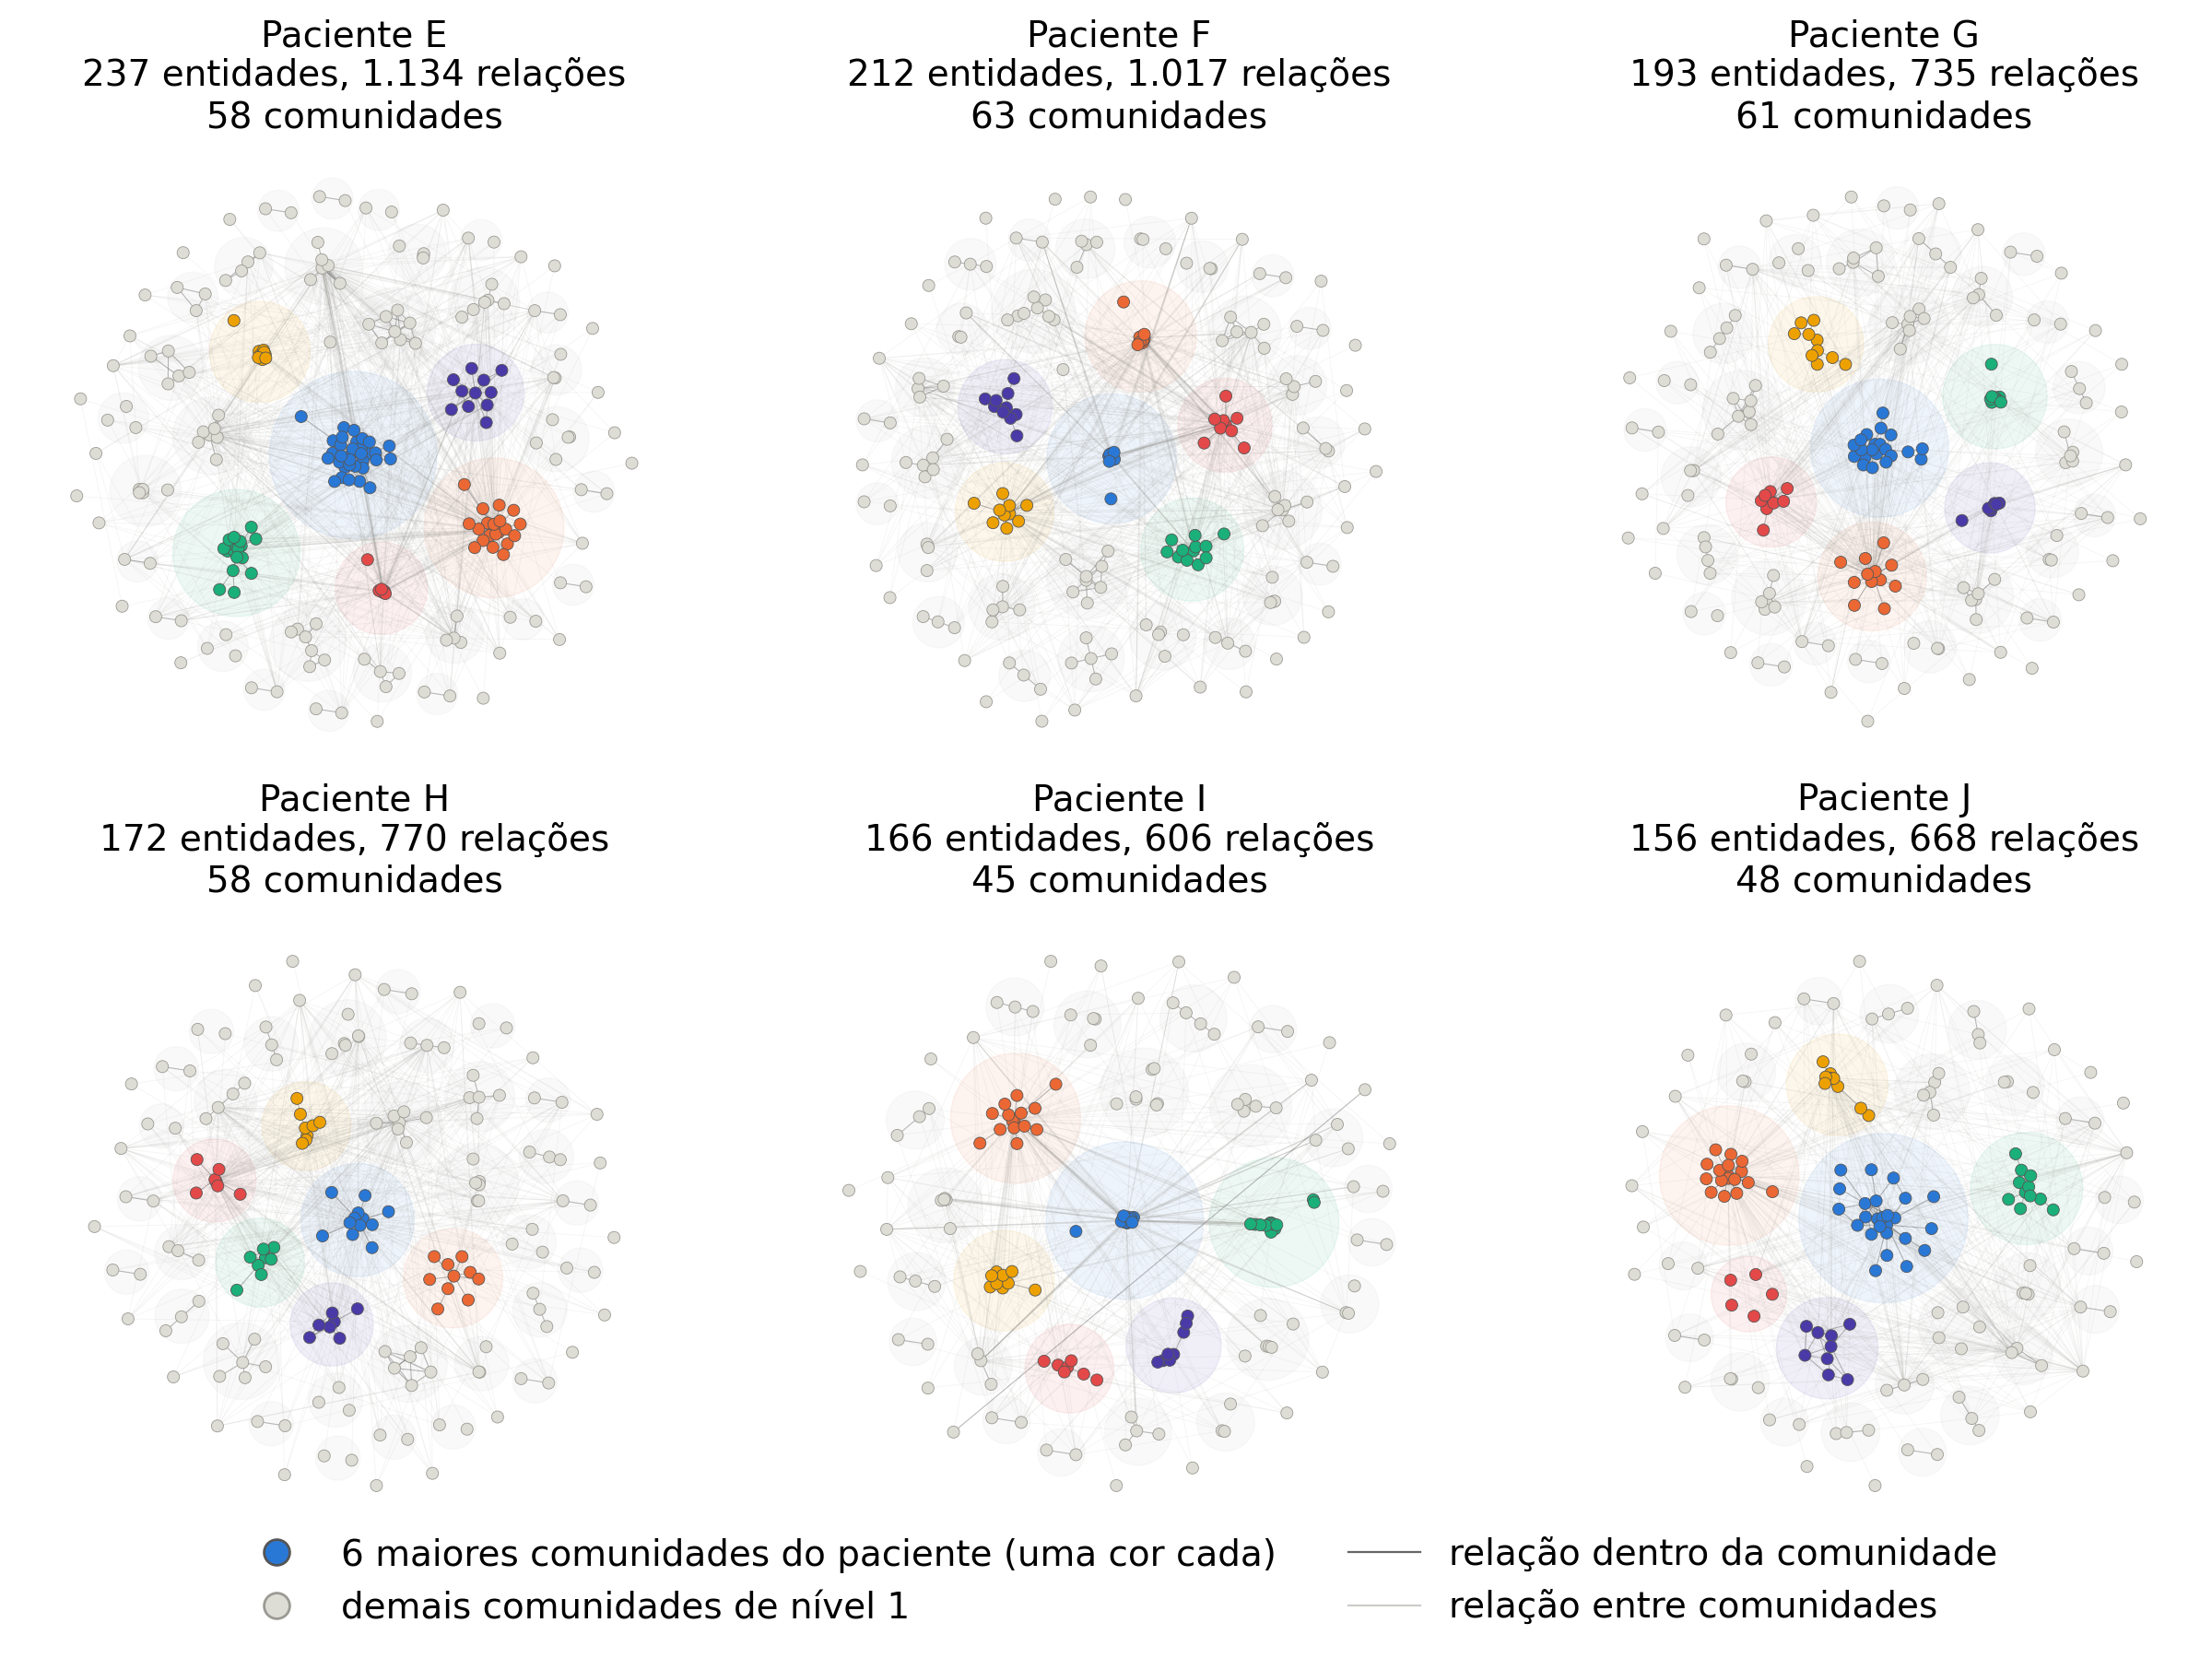
\includegraphics[width=\textwidth]{Cap05/figuras/comparacao_maiores_grafos.png}
\caption[Comparação dos seis maiores subgrafos da amostra]{Os seis maiores subgrafos da amostra, em número de entidades (pacientes E a J), com as entidades agrupadas por comunidade de nível 1; as seis maiores comunidades de cada paciente aparecem em cores, e as demais, em cinza.}
\label{fig:res-maiores-grafos}
\par\smallskip{\footnotesize Fonte: elaborado pelo autor com as bibliotecas NetworkX e matplotlib.}
\end{figure}

\FloatBarrier
\section{Síntese dos resultados}\label{sec:res-sintese}

Em conjunto, os resultados deste capítulo sustentam três conclusões. Primeira, o modo \textit{drift} supera \textit{basic} e \textit{local} em F1 macro, mas o ganho é assimétrico: decorre de uma revocação muito mais alta, e não de maior precisão, de modo que a escolha do sistema deve considerar explicitamente essa troca, e não apenas o valor agregado de F1. Segunda, o ganho do \textit{drift} concentra-se nas doenças que exigem inferência a partir de evidência indireta e dispersa no texto (cirrose, hipertensão portal, esquistossomose), enquanto é marginal nas doenças com marcador textual direto (hepatite B, hepatite C, esteatose), por efeito-teto, e inexistente em HDA, cujo padrão de erro é qualitativamente distinto: confusão anatômica entre sangramento alto e baixo, estatisticamente confirmada. Terceira, a diferença entre os níveis de comunidade 1 e 2 é pequena diante da diferença entre modos de busca: a maior delas, no \textit{drift}, foi de 0,053 de F1 macro, inferior à diferença entre \textit{basic} e \textit{drift} em qualquer dos dois níveis.

\begin{figure}[!htb]
\centering
% Gerado por experiments/grid_search/gera_figuras_tikz_tese.py -- não editar à mão
\begin{tikzpicture}
\begin{groupplot}[
  group style={group size=2 by 2, horizontal sep=1.6cm, vertical sep=1.9cm},
  width=0.5\textwidth, height=5.2cm,
  tick label style={font=\scriptsize}, label style={font=\footnotesize},
  title style={font=\footnotesize\bfseries, yshift=-1mm},
  axis lines=left, axis line style={black!45}, tick style={black!45},
  ymajorgrids, grid style={black!10}, ymin=0,
  /pgf/number format/use comma, /pgf/number format/1000 sep={.},
]
\nextgroupplot[title={Entidades por prontuário}, xlabel={Entidades}, ylabel={Prontuários}]
\addplot[ybar interval, fill opacity=1, draw=white, line width=0.3pt, fill=vAzul] coordinates {(5,12) (12.73,56) (20.47,109) (28.2,77) (35.93,57) (43.67,52) (51.4,39) (59.13,20) (66.87,26) (74.6,11) (82.33,13) (90.07,9) (97.8,14) (105.5,10) (113.3,4) (121,6) (128.7,8) (136.5,2) (144.2,2) (151.9,4) (159.7,1) (167.4,1) (175.1,0) (182.9,0) (190.6,1) (198.3,0) (206.1,1) (213.8,0) (221.5,0) (229.3,1) (237,0)};
\nextgroupplot[title={Relações por prontuário}, xlabel={Relações}, ylabel={Prontuários}]
\addplot[ybar interval, fill opacity=1, draw=white, line width=0.3pt, fill=vLaranja] coordinates {(4,110) (41.67,151) (79.33,76) (117,55) (154.7,30) (192.3,23) (230,12) (267.7,10) (305.3,8) (343,11) (380.7,8) (418.3,8) (456,5) (493.7,7) (531.3,6) (569,7) (606.7,2) (644.3,2) (682,0) (719.7,2) (757.3,1) (795,0) (832.7,0) (870.3,0) (908,0) (945.7,0) (983.3,1) (1021,0) (1059,0) (1096,1) (1134,0)};
\nextgroupplot[title={Entidades $\times$ relações}, xlabel={Entidades}, ylabel={Relações}, xmin=0]
\addplot[only marks, mark=*, mark size=1.1pt, color=vVerde, fill opacity=0.45, draw opacity=0] coordinates {(36,79) (28,48) (56,183) (41,135) (13,23) (37,69) (29,36) (26,31) (40,138) (37,70) (93,420) (106,285) (90,337) (130,527) (85,278) (112,289) (25,95) (17,27) (65,201) (58,136) (63,201) (143,733) (101,438) (56,168) (72,185) (24,48) (193,735) (61,174) (135,594) (24,49) (110,474) (36,61) (73,184) (69,261) (97,358) (45,103) (212,1017) (114,560) (99,499) (69,205) (30,42) (113,472) (49,220) (34,69) (237,1134) (46,80) (32,44) (55,210) (36,79) (103,496) (104,351) (108,412) (128,438) (124,585) (94,358) (110,435) (71,172) (69,230) (166,606) (69,187) (39,142) (55,134) (105,419) (119,487) (45,133) (122,297) (135,594) (124,629) (156,668) (68,158) (129,473) (148,522) (91,293) (131,543) (34,48) (65,141) (113,523) (125,507) (41,93) (31,57) (51,154) (111,448) (74,188) (120,266) (155,546) (41,92) (87,226) (154,533) (67,193) (25,41) (67,197) (76,239) (35,61) (45,78) (38,83) (24,51) (23,45) (19,42) (28,40) (21,33) (16,16) (35,96) (21,45) (30,67) (50,146) (45,180) (61,185) (50,160) (16,11) (35,77) (21,56) (28,39) (28,67) (23,57) (59,179) (34,38) (34,38) (46,135) (63,224) (33,70) (58,135) (49,169) (45,110) (50,87) (10,9) (33,57) (33,57) (53,129) (72,151) (30,77) (23,40) (29,54) (48,122) (41,107) (23,45) (54,142) (26,44) (56,132) (28,43) (28,42) (27,50) (33,44) (61,180) (28,46) (28,52) (19,37) (21,48) (55,136) (62,201) (43,104) (47,79) (19,46) (34,56) (26,53) (48,136) (19,34) (38,73) (41,93) (31,69) (51,195) (24,43) (32,72) (24,62) (32,47) (17,30) (22,23) (21,44) (31,62) (27,64) (21,42) (19,44) (38,58) (19,41) (32,81) (79,217) (19,28) (25,46) (20,38) (41,115) (21,44) (39,103) (40,97) (13,19) (25,35) (21,37) (32,64) (28,33) (22,42) (53,102) (52,115) (47,128) (50,134) (10,9) (27,63) (49,154) (35,92) (53,90) (25,74) (32,53) (27,61) (26,60) (43,130) (17,48) (25,35) (25,35) (52,189) (68,215) (24,50) (34,102) (59,151) (21,31) (24,76) (29,48) (83,250) (41,147) (30,59) (29,65) (45,73) (25,68) (18,23) (18,21) (41,114) (32,71) (17,19) (5,4) (21,25) (9,5) (29,36) (23,35) (30,102) (56,144) (18,29) (35,76) (34,70) (22,39) (54,139) (32,53) (50,153) (24,49) (36,81) (30,80) (59,174) (31,54) (21,32) (37,90) (42,108) (17,22) (27,65) (26,52) (16,20) (31,93) (23,36) (45,97) (14,15) (27,36) (26,45) (57,168) (16,18) (16,18) (13,8) (27,59) (27,59) (29,39) (27,51) (38,68) (45,99) (15,23) (42,85) (13,11) (47,103) (32,30) (30,49) (7,9) (68,260) (30,66) (16,25) (21,40) (21,40) (18,31) (47,82) (66,149) (47,99) (21,35) (23,82) (44,151) (25,42) (18,46) (25,24) (29,44) (53,136) (20,20) (37,85) (44,92) (30,52) (27,48) (13,15) (45,102) (18,17) (8,7) (20,45) (25,59) (20,26) (29,41) (42,78) (32,53) (9,8) (21,25) (49,104) (31,42) (18,16) (38,82) (64,182) (12,11) (39,81) (39,113) (30,50) (31,74) (29,75) (40,79) (40,79) (45,80) (23,40) (44,75) (29,45) (26,44) (48,92) (31,82) (14,23) (51,129) (25,48) (20,45) (13,20) (23,54) (41,158) (29,76) (33,77) (52,134) (43,135) (28,40) (28,46) (29,78) (47,147) (28,86) (56,218) (19,19) (16,17) (49,117) (17,23) (19,40) (20,32) (26,43) (22,32) (21,29) (27,58) (18,31) (33,84) (16,20) (10,13) (58,207) (20,26) (34,56) (22,39) (23,63) (22,29) (10,13) (56,149) (37,86) (28,34) (29,58) (102,366) (78,284) (53,121) (98,348) (43,71) (51,140) (100,395) (97,326) (34,52) (68,156) (94,343) (71,193) (63,169) (23,47) (38,57) (73,133) (12,13) (35,69) (27,78) (36,56) (100,357) (32,64) (85,392) (45,69) (22,28) (35,53) (35,102) (23,29) (155,387) (46,112) (82,361) (131,592) (25,26) (94,311) (74,209) (52,137) (31,73) (60,145) (172,770) (50,123) (95,420) (48,157) (81,308) (83,293) (73,251) (42,79) (31,55) (39,102) (16,20) (82,392) (34,46) (67,174) (100,272) (16,23) (62,111) (102,466) (42,103) (66,215) (62,171) (47,86) (87,315) (41,131) (41,101) (28,51) (26,90) (53,130) (43,100) (87,449) (41,67) (32,62) (61,165) (66,210) (36,67) (73,176) (85,407) (24,54) (57,81) (117,316) (49,135) (73,226) (107,385) (43,73) (31,104) (134,544) (43,87) (49,166) (146,520) (55,149) (82,315) (111,555) (124,616) (136,577) (26,47) (100,578) (40,69) (52,122) (80,302) (46,94) (67,179) (58,127) (27,77) (85,240) (56,149) (41,98) (33,85) (79,355) (71,211) (32,74) (81,389) (68,266) (38,105) (61,182) (31,60) (20,30) (87,352) (24,60) (24,27) (90,317) (65,204) (44,128) (32,84) (52,88) (20,36) (99,283) (19,19) (31,59) (60,125) (45,102) (14,16) (69,250) (17,28) (27,38) (42,85) (95,246) (54,106) (51,133) (143,654) (25,54) (39,74) (25,69) (45,137) (42,98) (26,38) (8,10) (26,61) (27,45) (32,81) (21,32) (53,91) (36,84) (23,40) (45,75) (103,350) (57,94) (88,201) (75,252) (13,13) (59,137) (54,149) (32,44) (24,29) (28,95) (24,38) (18,18) (44,97) (22,32) (26,47)};
\node[anchor=north west, font=\scriptsize, fill=white, inner sep=2pt] at (rel axis cs:0.03,0.97) {$r = 0{,}959$};
\nextgroupplot[title={Comunidades distintas por prontuário}, xlabel={Comunidades distintas (nível 1)}, ylabel={Prontuários}]
\addplot[ybar interval, fill opacity=1, draw=white, line width=0.3pt, fill=vRoxo] coordinates {(0,1) (1,0) (2,0) (3,0) (4,0) (5,2) (6,3) (7,3) (8,5) (9,6) (10,9) (11,18) (12,16) (13,24) (14,16) (15,29) (16,27) (17,21) (18,26) (19,30) (20,20) (21,22) (22,15) (23,23) (24,21) (25,19) (26,13) (27,10) (28,12) (29,14) (30,6) (31,19) (32,8) (33,11) (34,8) (35,6) (36,10) (37,8) (38,5) (39,9) (40,2) (41,3) (42,5) (43,3) (44,4) (45,3) (46,2) (47,1) (48,3) (49,2) (50,0) (51,3) (52,3) (53,0) (54,1) (55,0) (56,0) (57,1) (58,2) (59,0) (60,1) (61,1) (62,0) (63,1) (64,0)};
\end{groupplot}
\end{tikzpicture}

\caption[Distribuição estrutural dos subgrafos por prontuário]{Entidades, relações e comunidades por prontuário, e correlação entre entidades e relações.}
\label{fig:res-estrutura-agregada}
\par\smallskip{\footnotesize Fonte: elaborado pelo autor a partir do índice construído.}
\end{figure}
